\documentclass[12pt,letterpaper]{article}

%\usepackage{cogsci}
\usepackage[margin=1in]{geometry}
\usepackage{setspace}
\usepackage{pslatex}
\usepackage{apacite}
\usepackage{subfig}
\usepackage{graphicx}
\usepackage[english]{babel}
\usepackage{grffile}
\usepackage{amsmath, amsthm, amssymb}

\abovecaptionskip=5pt           % space between figure and caption
\belowcaptionskip=3pt plus 1pt  % space after caption except for bottom figure
\intextsep=2pt plus 1pt         % space between [h]ere figure and text
\textfloatsep=2pt plus 1pt      % space between [t]op or [b]ottom figure & text 

\newenvironment{packed_enum}{
\begin{enumerate}
  \setlength{\itemsep}{1pt}
  \setlength{\parskip}{0pt}
  \setlength{\parsep}{0pt}
}{\end{enumerate}}

\setlength{\abovecaptionskip}{.1in}
\setlength{\belowcaptionskip}{.25in}

\title{PyStoch: An Implementation of Stochastic Python}
\author{Jessica Hamrick (\texttt{jhamrick@mit.edu})}
\date{\today{}}

\begin{document}

\newcommand{\TODO}[1]{[TODO: #1]}

\maketitle
\doublespacing

\section{Introduction}
\label{sec:introduction}

Probabilistic programming is a recent development in the field of
Bayesian inference.  A probabilistic programming language is a
framework layered on top of a pre-existing language such as Church
\cite{Goodman2008} or Matlab \cite{Wingate2011} that allows the
programmer to easily implement probabilistic models.  The programmer
specifies a computation to be performed and a condition indicating
when a value of the computation should be accepted.  The power of
probabilistic programs comes from their ability to abstract the design
of the model away from the implementation of the inference.  Instead
of having to program his or her own implementation of, for example,
the Metropolis-Hastings algorithm for Markov Chain Monte Carlo
sampling, the researcher can simply code the structure of the model
and leave the inference to the probabilistic programming language.

Scheme and Matlab are both extremely useful languages, yet both are
confined to relatively small niches in the world of programming
languages.  Other languages such as Python are widely used and many
libraries exist for nearly every aspect of coding.  Creating a
stochastic version of Python would be immensely useful, as it would
provide integration of these external libraries with the powerful
inference of a probabilistic programming language.  \citeA{Wingate2011}
developed a framework for easily creating new probabilistic
programming languages, and this project uses this framework to present
an implementation of stochastic Python, henceforth known as
PyStoch\footnote{The source code and documentation for PyStoch can be
  found at https://github.com/jhamrick/pystoch}.

\section{Approach}

\citeA{Wingate2011} present two methods of creating a probabilistic
programming language, one being functional and the second imperative.
While Python incorporates both functional and imperative programming
styles, it is ultimately a more imperative programming language.  To
accommodate this, the imperative method of creating a probabilistic
programming language is used.


\begin{figure}
\begin{verbatim}
import numpy as np

def foo():
    samples = [np.random.randn() for x in xrange(100)]
    foomean = np.mean(foo)
    foostd = np.std(foo)
    print "%s +/- %s" % (foomean, foostd)
    return foomean, foostd
\end{verbatim}
\caption{\small\textbf{A Simple Python Program.}  This is a simple
  python program that draws 100 random samples from a standard normal
  distribution, calculates their mean and standard deviation, prints
  the mean and standard deviation, and finally returns both values in
  a tuple.  Fig. \ref{fig:compiled} shows the same program compiled
  into PyStoch source code.}
\label{fig:source}
\end{figure}

\begin{figure}
\begin{verbatim}
PYSTOCHOBJ.line_stack.push(0)
PYSTOCHOBJ.line_stack.set(1)
import numpy as np

def foo(PYSTOCHOBJ=None):
    PYSTOCHOBJ.func_stack.push('PYSTOCHID_7175f21c')
    PYSTOCHOBJ.line_stack.push(0)
    PYSTOCHOBJ.line_stack.set(1)
    PYSTOCHID_318c5560 = []
    PYSTOCHOBJ.line_stack.set(2)
    PYSTOCHOBJ.loop_stack.push(0)
    for x in PYSTOCHOBJ.call(xrange, 100):
        PYSTOCHOBJ.loop_stack.increment()
        PYSTOCHOBJ.line_stack.set(3)
        PYSTOCHID_26d0fb2a = PYSTOCHOBJ.call(np.random.randn)
        PYSTOCHOBJ.line_stack.set(4)
        PYSTOCHOBJ.call(PYSTOCHID_318c5560.append, PYSTOCHID_26d0fb2a)
    PYSTOCHOBJ.loop_stack.pop()
    PYSTOCHOBJ.line_stack.set(5)
    samples = PYSTOCHID_318c5560
    PYSTOCHOBJ.line_stack.set(6)
    foomean = PYSTOCHOBJ.call(np.mean, foo)
    PYSTOCHOBJ.line_stack.set(7)
    foostd = PYSTOCHOBJ.call(np.std, foo)
    PYSTOCHOBJ.line_stack.set(8)
    print ('%s +/- %s' % (foomean, foostd))
    PYSTOCHOBJ.line_stack.pop()
    PYSTOCHOBJ.func_stack.pop()
    return (foomean, foostd)
foo.random = True

PYSTOCHOBJ.line_stack.pop()
\end{verbatim}
\caption{\small\textbf{A Simple PyStoch Program.}  This is a simple
  Python program (see Fig. \ref{fig:source} compiled into PyStoch
  source code.  It draws 100 random samples from a standard normal
  distribution, calculates their mean and standard deviation, prints
  the mean and standard deviation, and finally returns both values in
  a tuple.}
\label{fig:compiled}
\end{figure}

\subsection{Metropolis-Hastings Trace Sampling}
\label{sec:mh}

\subsection{Compilation}
\label{sec:compilation}

In order to use the Metropolis-Hastings algorithm to perform inference
(see Sec. \ref{sec:mh}), it must be possible to identify all of the
random variables in a stochastic program.  The method by which this is
done is to rewrite the source code of the program to keep track of the
current function, loop iteration, and line for every point in the
program.  To do this, I used Python's abstract syntax tree module
\cite{ast} to perform a static analysis of the source code as detailed
by \citeA{Wingate2011}.  To output the transformed syntax tree back
into code, I used the \texttt{codegen} module written by Robert Kern
\cite{codegen}.  

Fig. \ref{fig:source} shows an example of a simple program, and
Fig. \ref{fig:compiled} shows the program transformed into PyStoch
source code.  Several things are important to note.  First, the
function is rewritten to take a parameter \texttt{PYSTOCHOBJ}.  This
variable keeps track of the function, line, and loop stacks, as well
as other information crucial to the Metropolis-Hastings algorithm (see
Sec. \ref{sec:mh}).  Second, all function calls are routed through the
\texttt{PYSTOCHOBJ}.  Because Python has first-class functions, it is
not possible to statically determine which functions are random and
which are not.  To deal with this issue, the \texttt{PYSTOCHOBJ}
handles function calls at run-time depending on their attributes.  One
such attribute is the \texttt{random} attribute; the \texttt{foo}
function has been augmented with this attribute to let
\texttt{PYSTOCHOBJ} know that when called, it should be passed a
reference of \texttt{PYSTOCHOBJ}.  Finally, iterative structures such
as list comprehensions are expanded, and there is at most one function
call per line.  This guarantees that there will never be any naming
conflicts for random function calls that happen to be on the same line
in the original source program.

\begin{figure}
\begin{verbatim}
class Query(MetropolisHastings):
    def __init__(self):
        ... initialization of the model ...

    def query_model(self):
        ... computation that is repeated during each trace of the
            Metropolis-Hastings algorithm ...

    def sample(self):
        ... return the value of variable(s) computed in query_model
            as the sample of the query ...

    def condition(self):
        ... return a boolean representing whether some condition has
            been met by the variable(s) computed in query model ...

samples = Query().run(num_samples, num_steps)
\end{verbatim}
  \caption{\small\textbf{Structure of a \texttt{MetropolisHastings}
      query.}  Models should inherit from the
    \texttt{MetropolisHastings} class and implement the methods as
    described.  The query is then run by calling the \texttt{run}
    method, passing in the number of samples to return and the number
    of iterations of the algorithm to run between samples.}
\label{fig:mh}
\end{figure}

\citeA{Wingate2011} give pseudo-code for an algorithm to use the
Metropolis-Hastings method, which has been implemented in PyStoch to
allow \texttt{MetropolisHastings} queries.  \citeA{Wingate2011} cites
several ways of initializing the \texttt{MetropolisHastings} algorithm
with a known set of values that match the condition; PyStoch's
implementation of the algorithm utilizes a \texttt{RejectionQuery} to
find a set of initial values.

A probabilistic program using the \texttt{MetropolisHastings} query
has the structure shown in Fig. \ref{fig:mh}.  All models wishing to
use the query must inherit from the \texttt{MetropolisHastings} class
and implement the \texttt{\_\_init\_\_}, \texttt{query\_model},
\texttt{sample}, and \texttt{condition} methods.

\section{Results}

To test the correctness of PyStoch's implementation of the
Metropolis-Hastings algorithm, samples were drawn from each of the
different ERP types: binomial, exponential, flip, gamma, Gaussian,
Poisson, discrete uniform (\texttt{sample\_integer}), and continuous
uniform.  Both the Metropolis-Hastings algorithm was used as well as a
simple implementation of \texttt{RejectionQuery} for comparison.
Fig. \ref{fig:erps} shows the histograms of drawing 1000 samples from
each distribution.  The shapes of the distributions are clearly
visible, and the histograms are consistent with each other as well as
the original distributions.

While verifying that basic distributions can be correctly sampled from
is important to prove the correctness of PyStoch, it does not give any
indication of how well PyStoch handles conditional inference.
Figs. \ref{fig:test1model}, \ref{fig:test2model},
\ref{fig:test3model}, \ref{fig:test4model}, and \ref{fig:test5model}
give the Python code for increasingly complex models, all taken from
the Church wiki.  In Fig. \ref{fig:test1model}, three random variables
taking on the values of either 0 or 1 are summed, and the model is
conditioned on their sum $D$ being greater than or equal to two.  The
model then returns the value of the first random variable, $A$, for
which $D\geq 2$ is true.  In Fig. \ref{fig:test2model}, probabilities
are defined for having breast cancer and for true and false positive
rates of mammograms.  The model then queries the probability of having
breast cancer given a positive mammogram.  Fig. \ref{fig:test3model}
defines the say that several different diseases and symptoms depend on
each other, and queries whether or not a patient has lunch cancer
and/or tuberculosis given that they have a cough, fever, chest pain,
and shortness of breath.  Fig. \ref{fig:test4model} queries the belief
about the weight of a coin given that five heads have been observed.
Finally, Fig. \ref{fig:test5model} asks whether or not a set of data
is more likely to have come from a large super set or a small super set.

\begin{figure}[t!]
\centering
\subfloat[Binomial ($n=20$, $p=0.8$)]{\label{fig:binomial}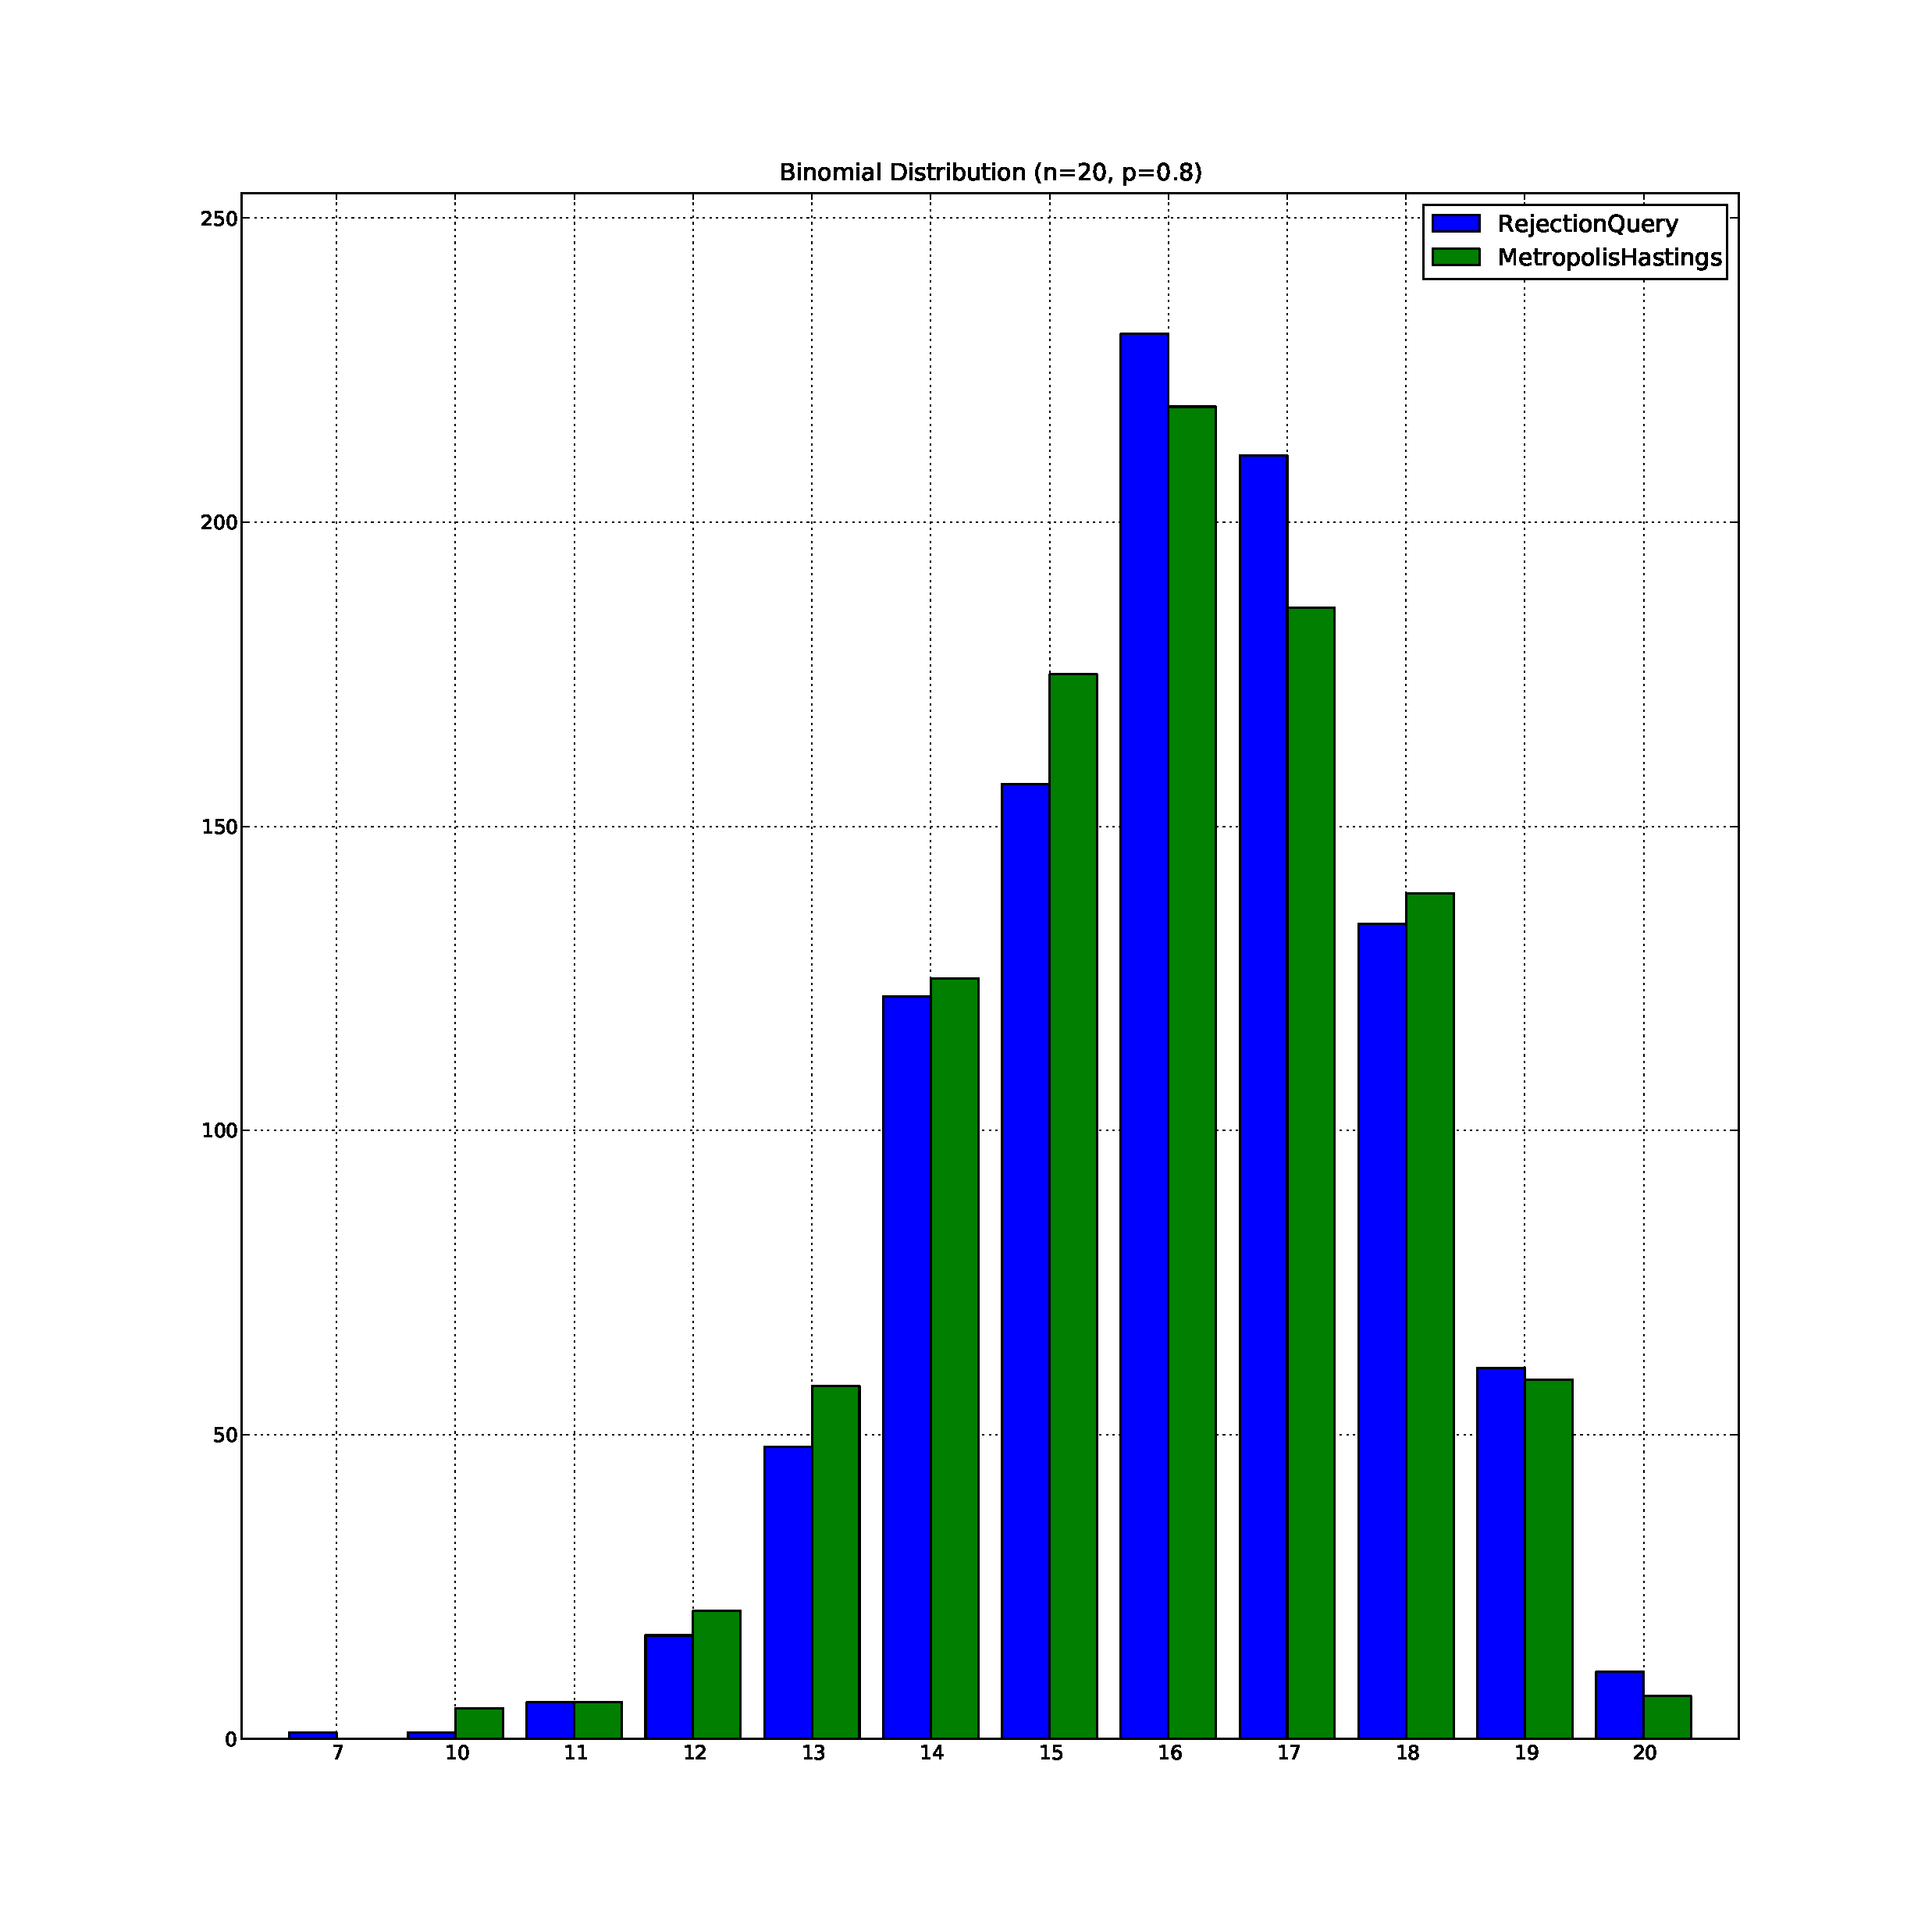
\includegraphics[width=0.33\textwidth]{../graphs/binomial.pdf}}
\subfloat[Exponential ($\lambda=0.5$)]{\label{fig:exponential}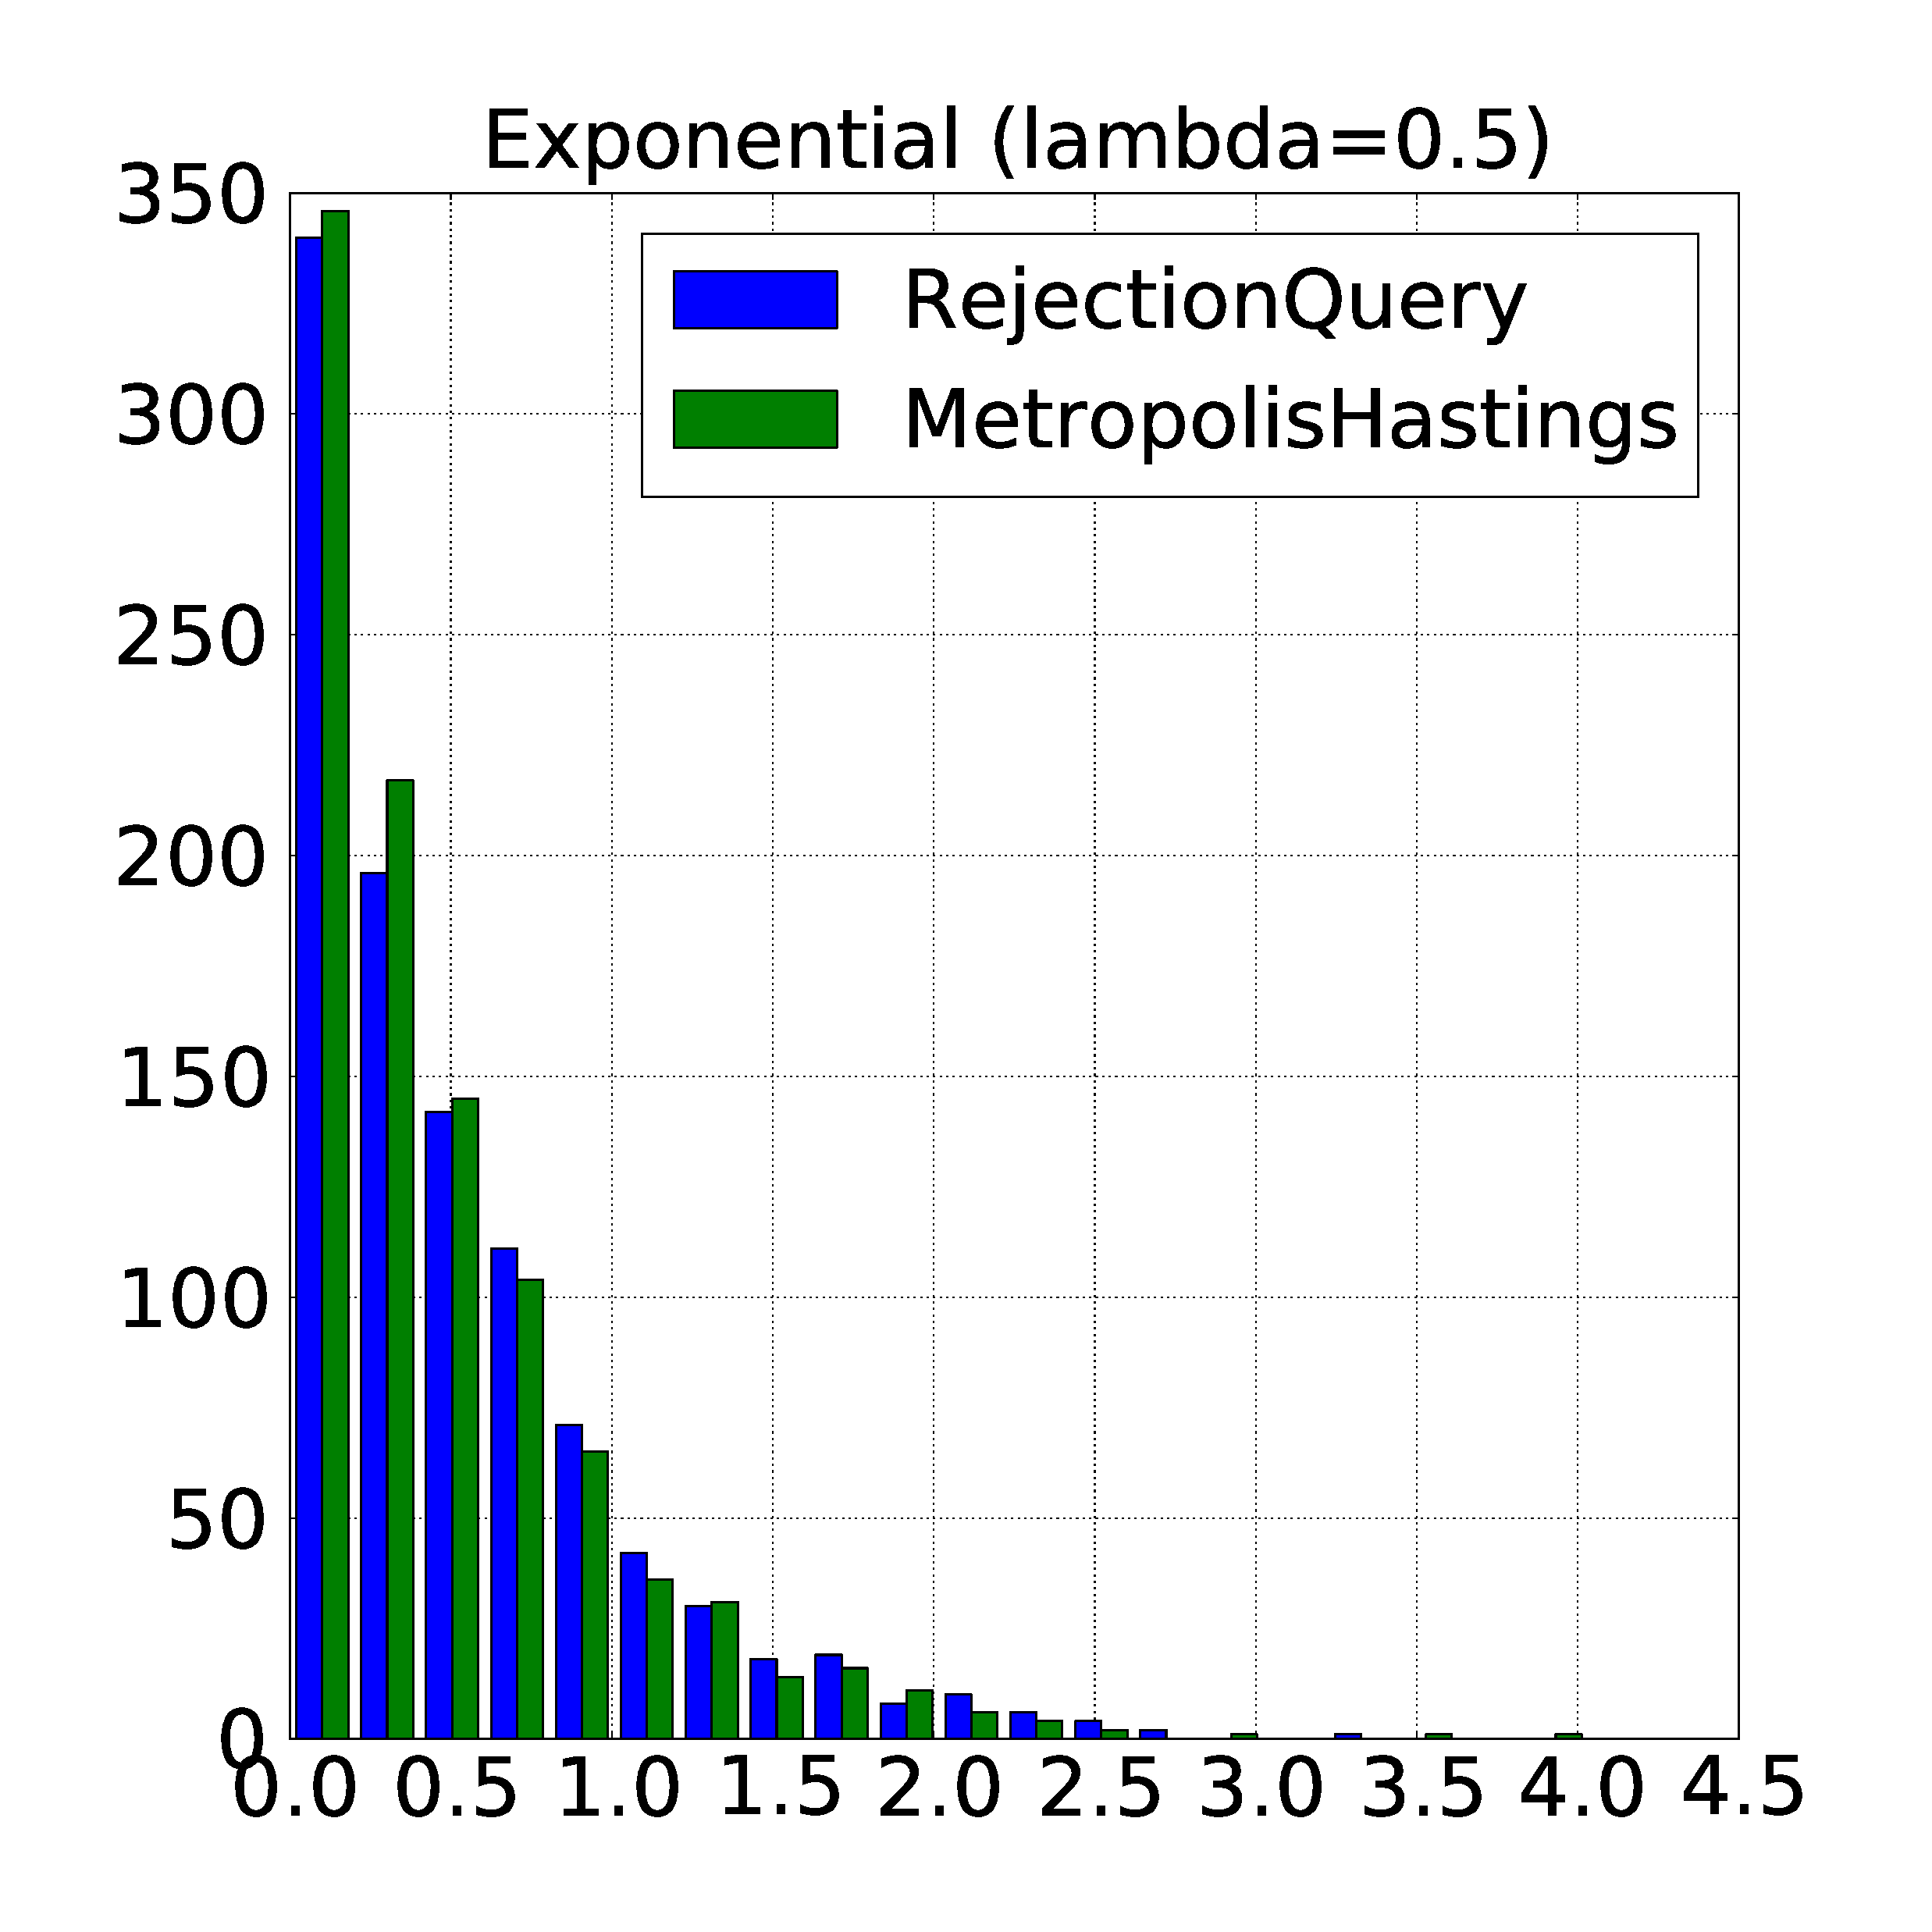
\includegraphics[width=0.33\textwidth]{../graphs/exponential.pdf}}
\subfloat[Flip ($w=0.5$)]{\label{fig:flip}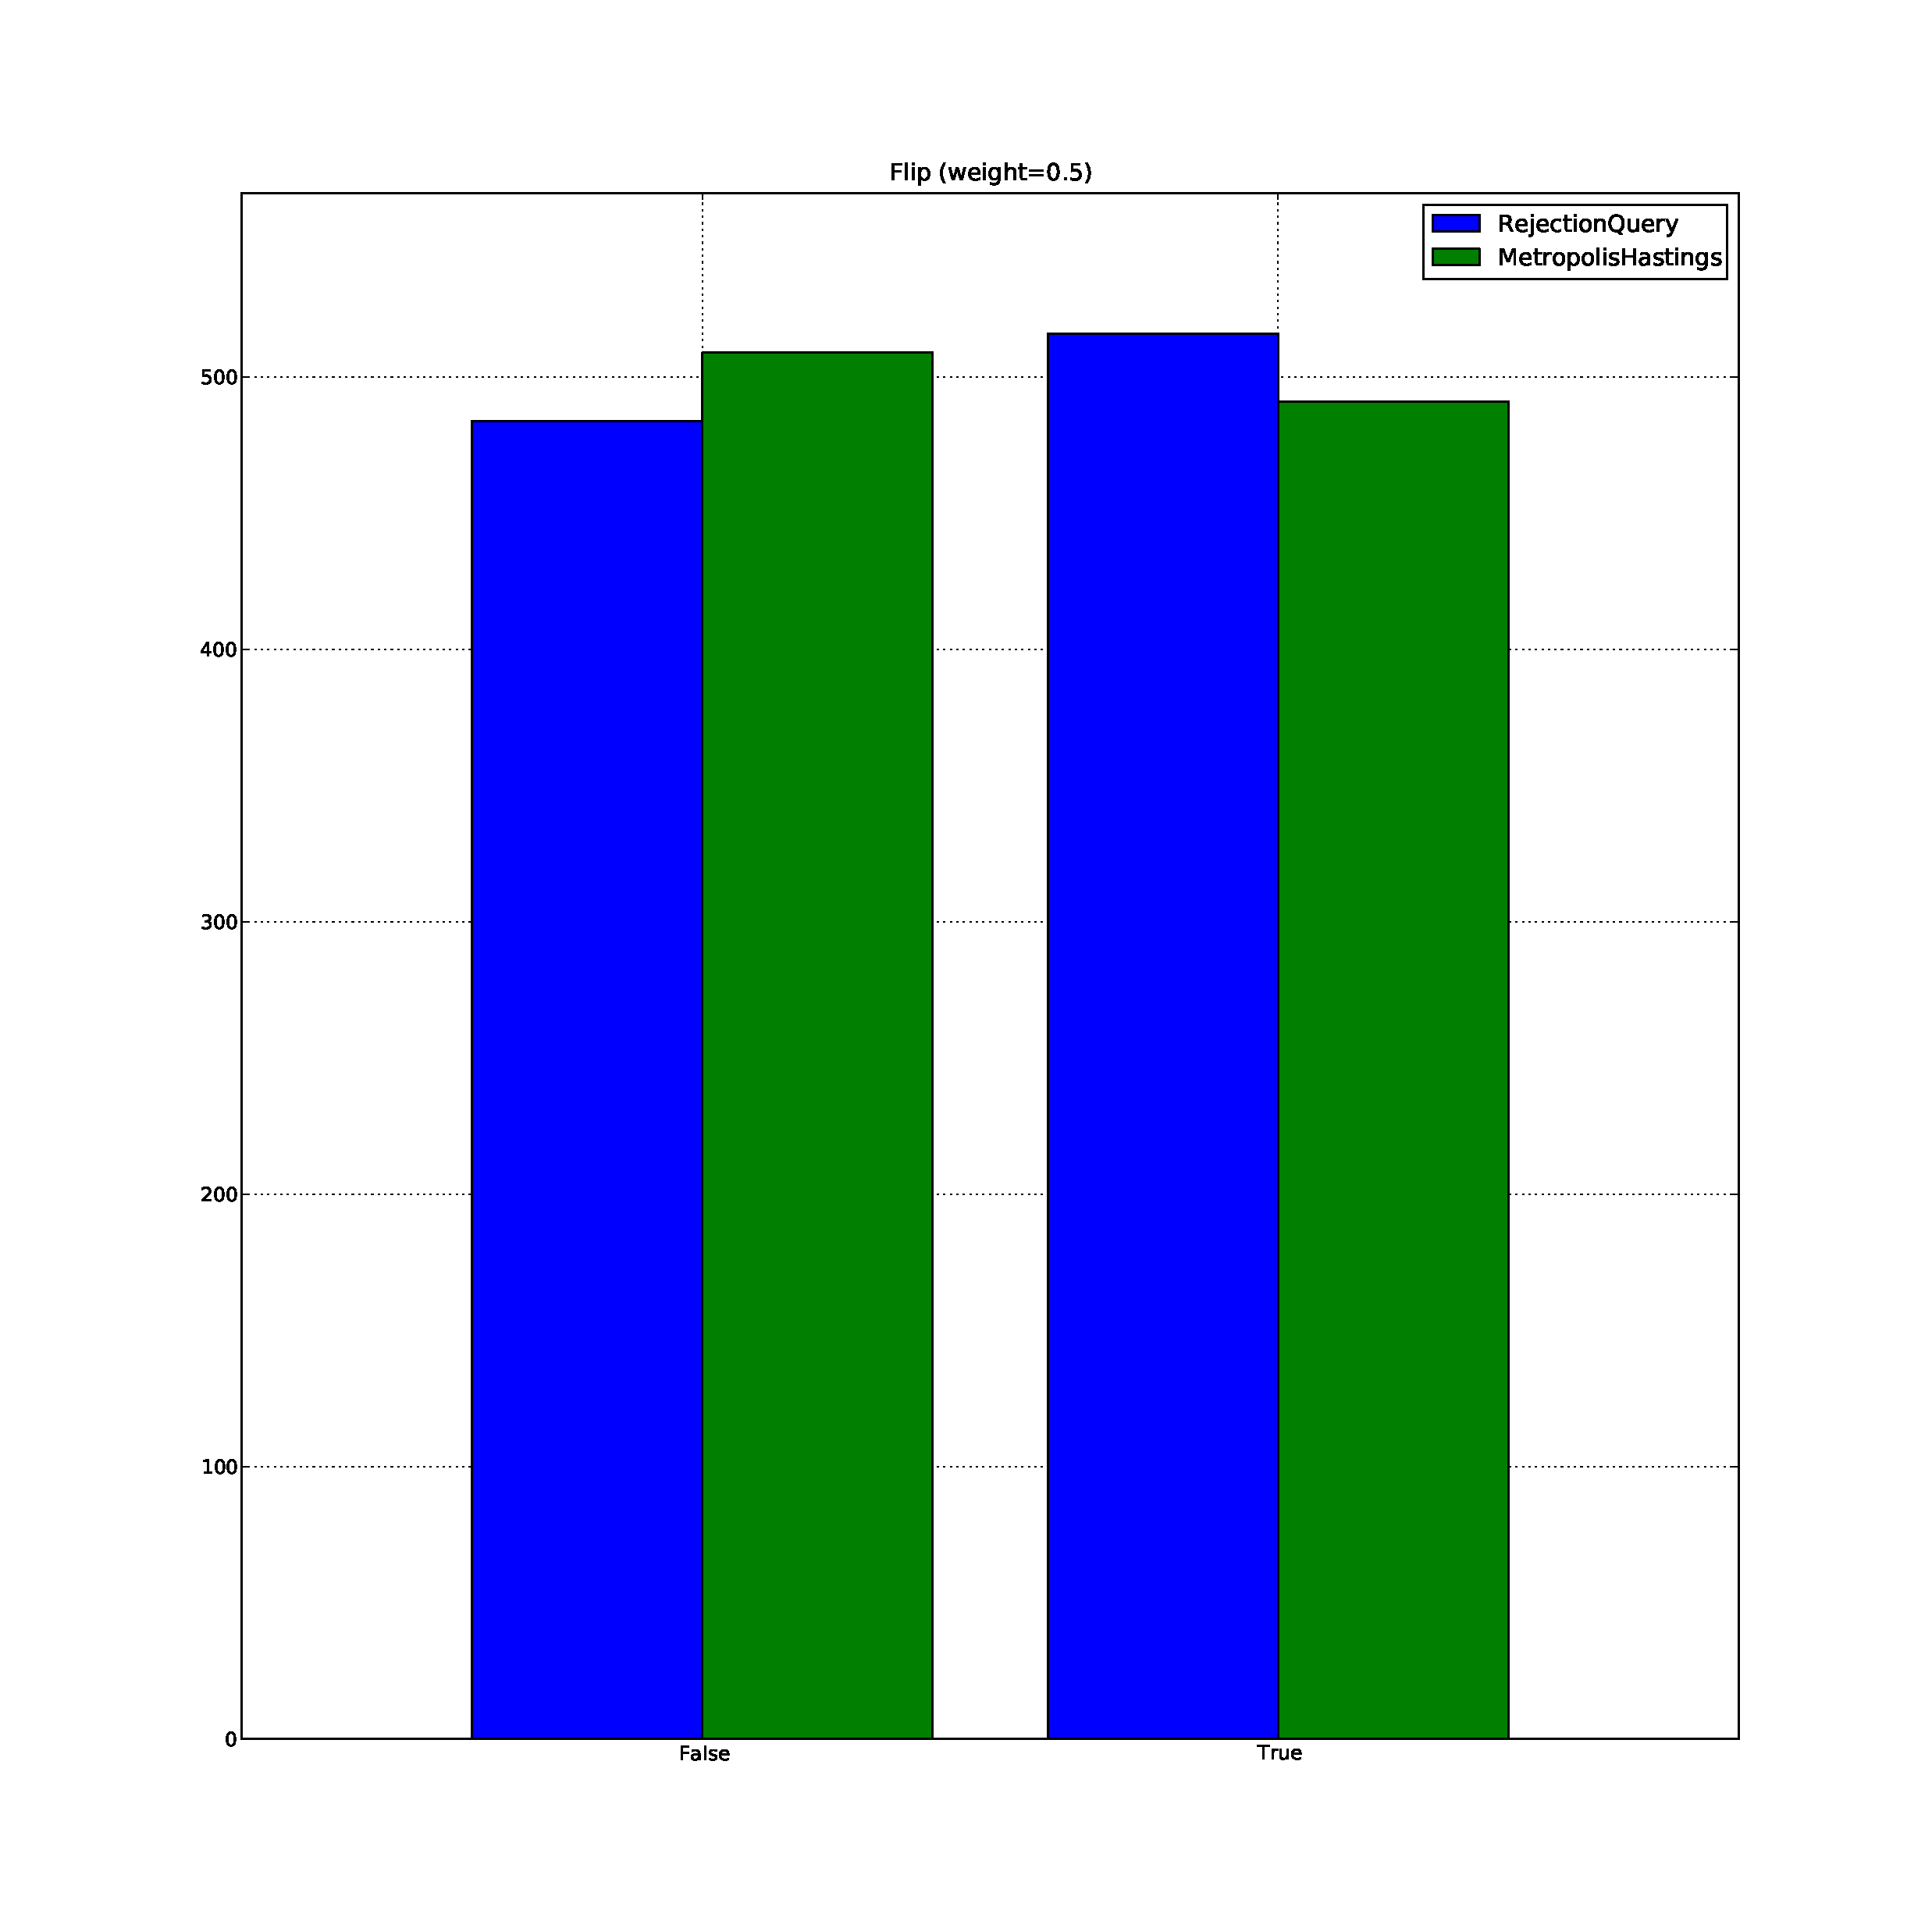
\includegraphics[width=0.33\textwidth]{../graphs/flip.pdf}}

\subfloat[Gamma ($k=2$, $\theta=2$)]{\label{fig:gamma}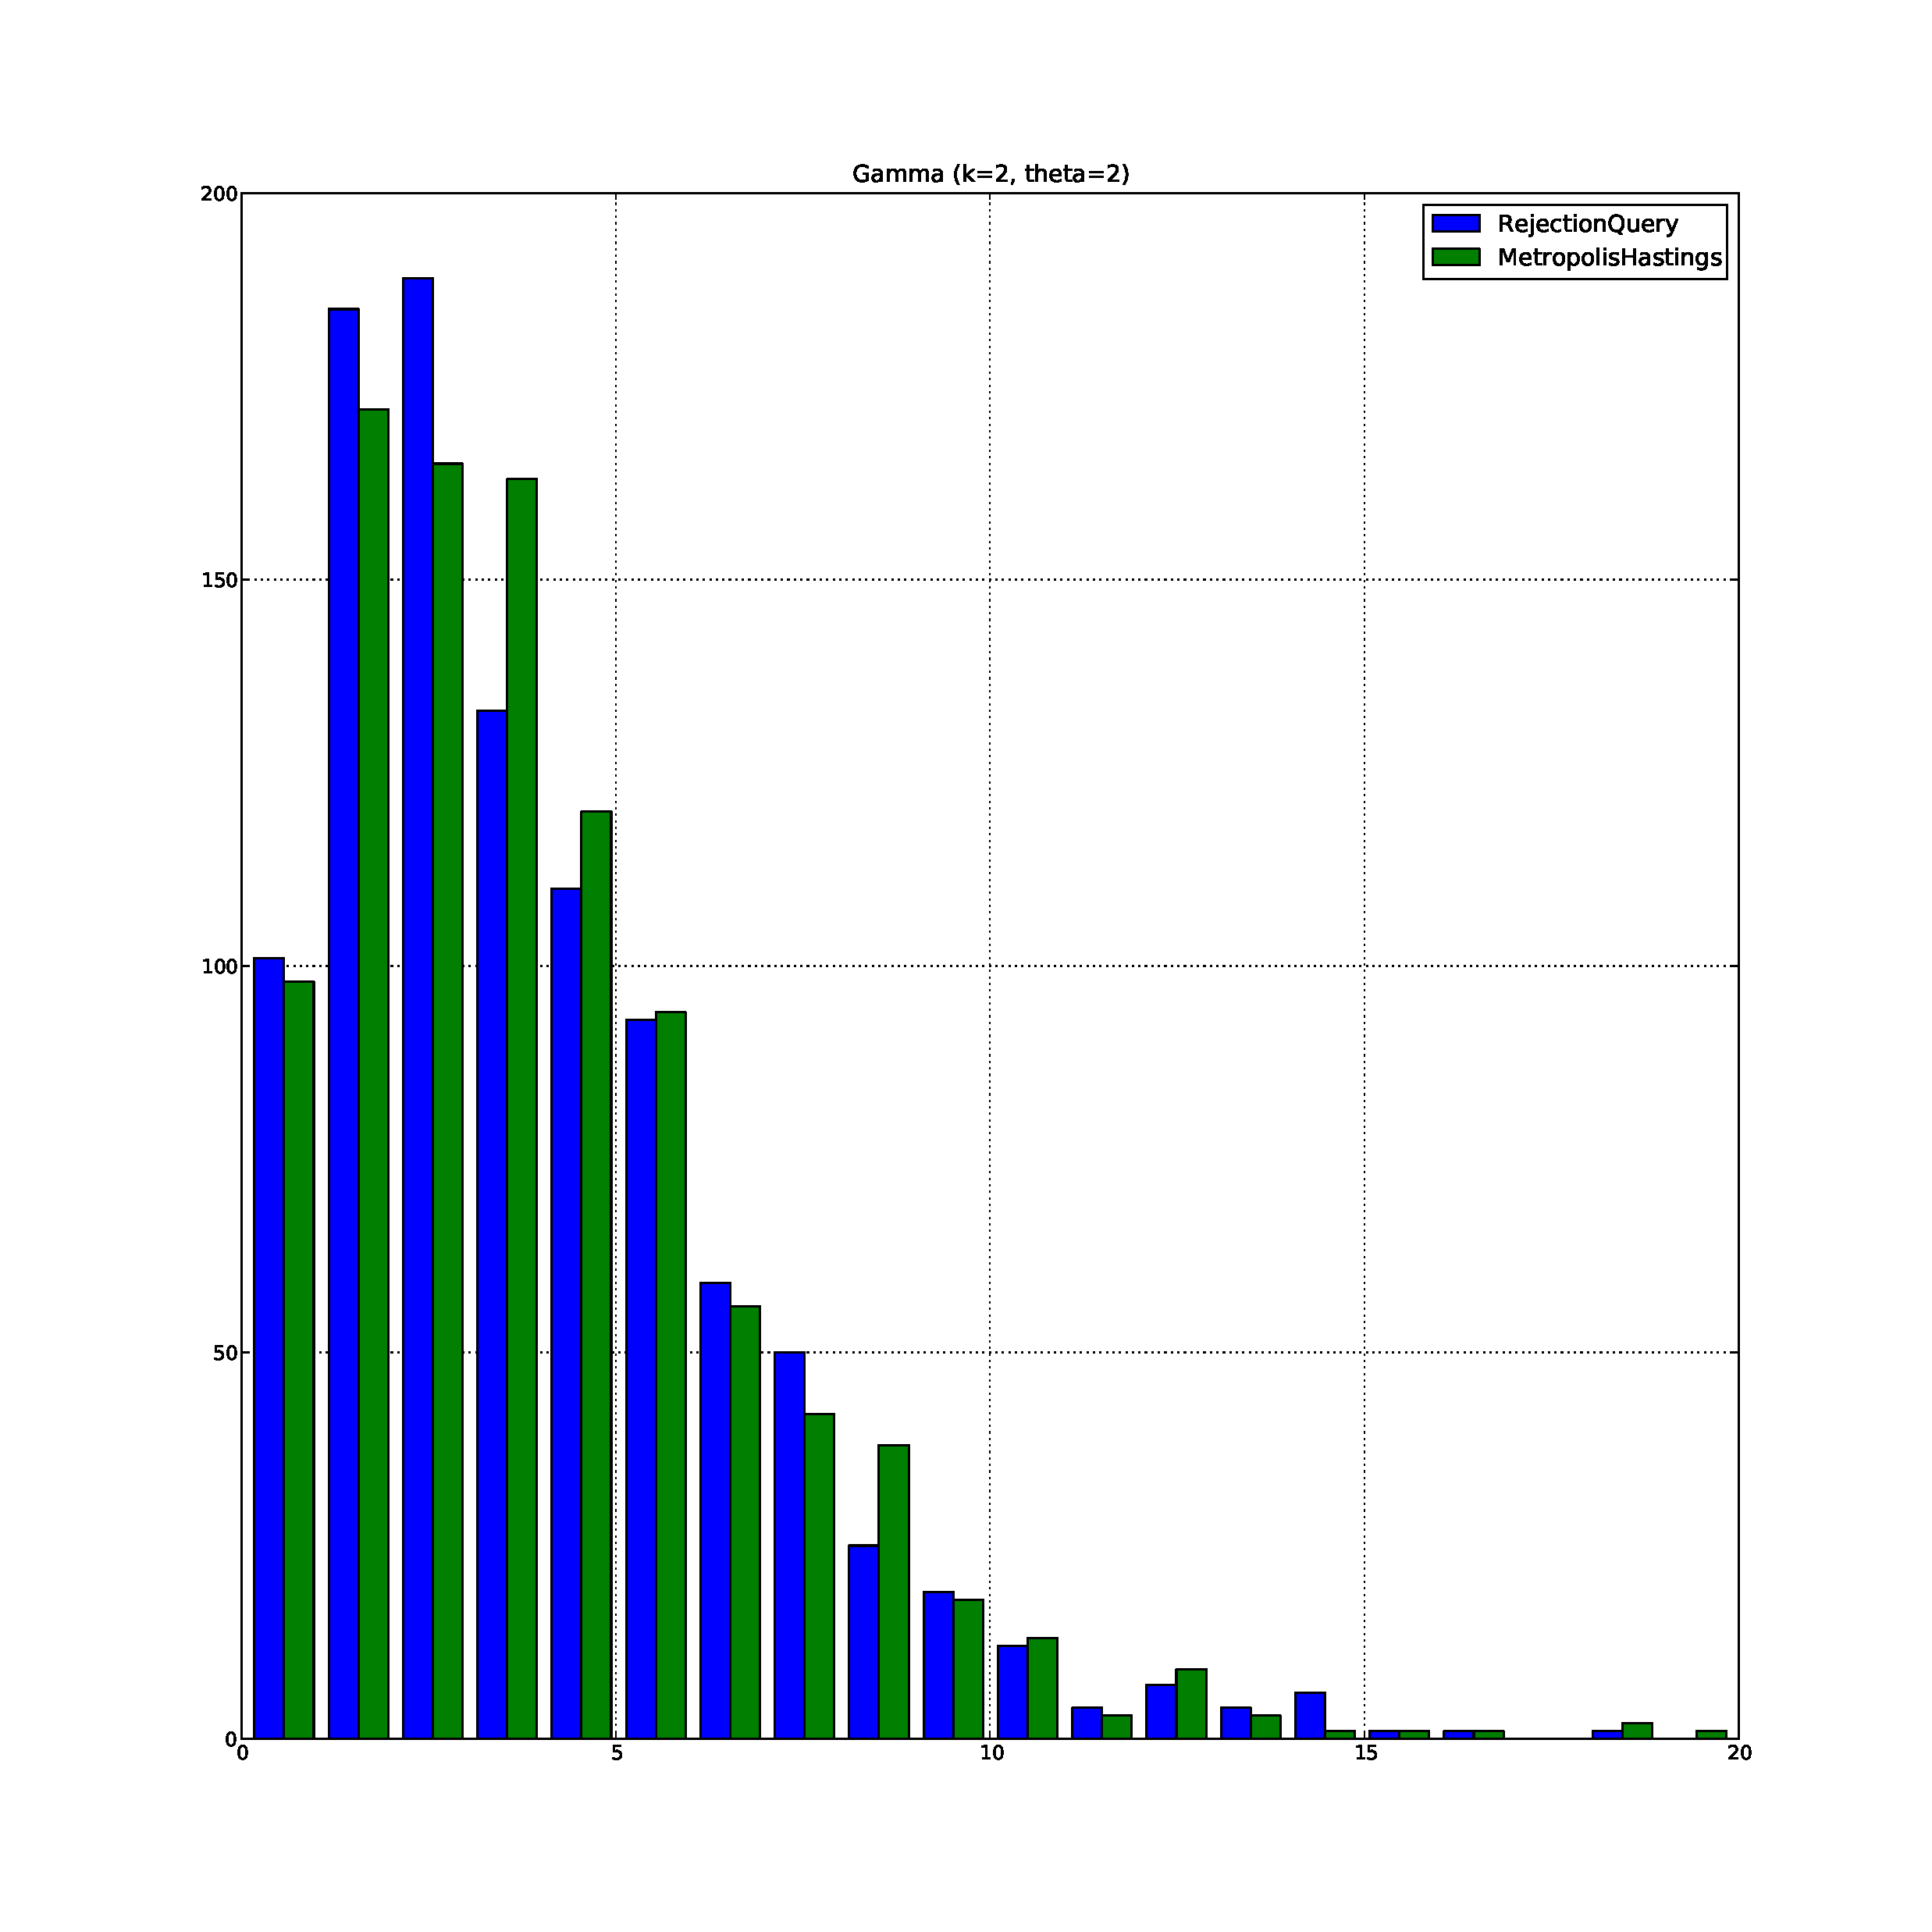
\includegraphics[width=0.33\textwidth]{../graphs/gamma.pdf}}
\subfloat[Gaussian ($\mu=0$, $\sigma=1$)]{\label{fig:gaussian}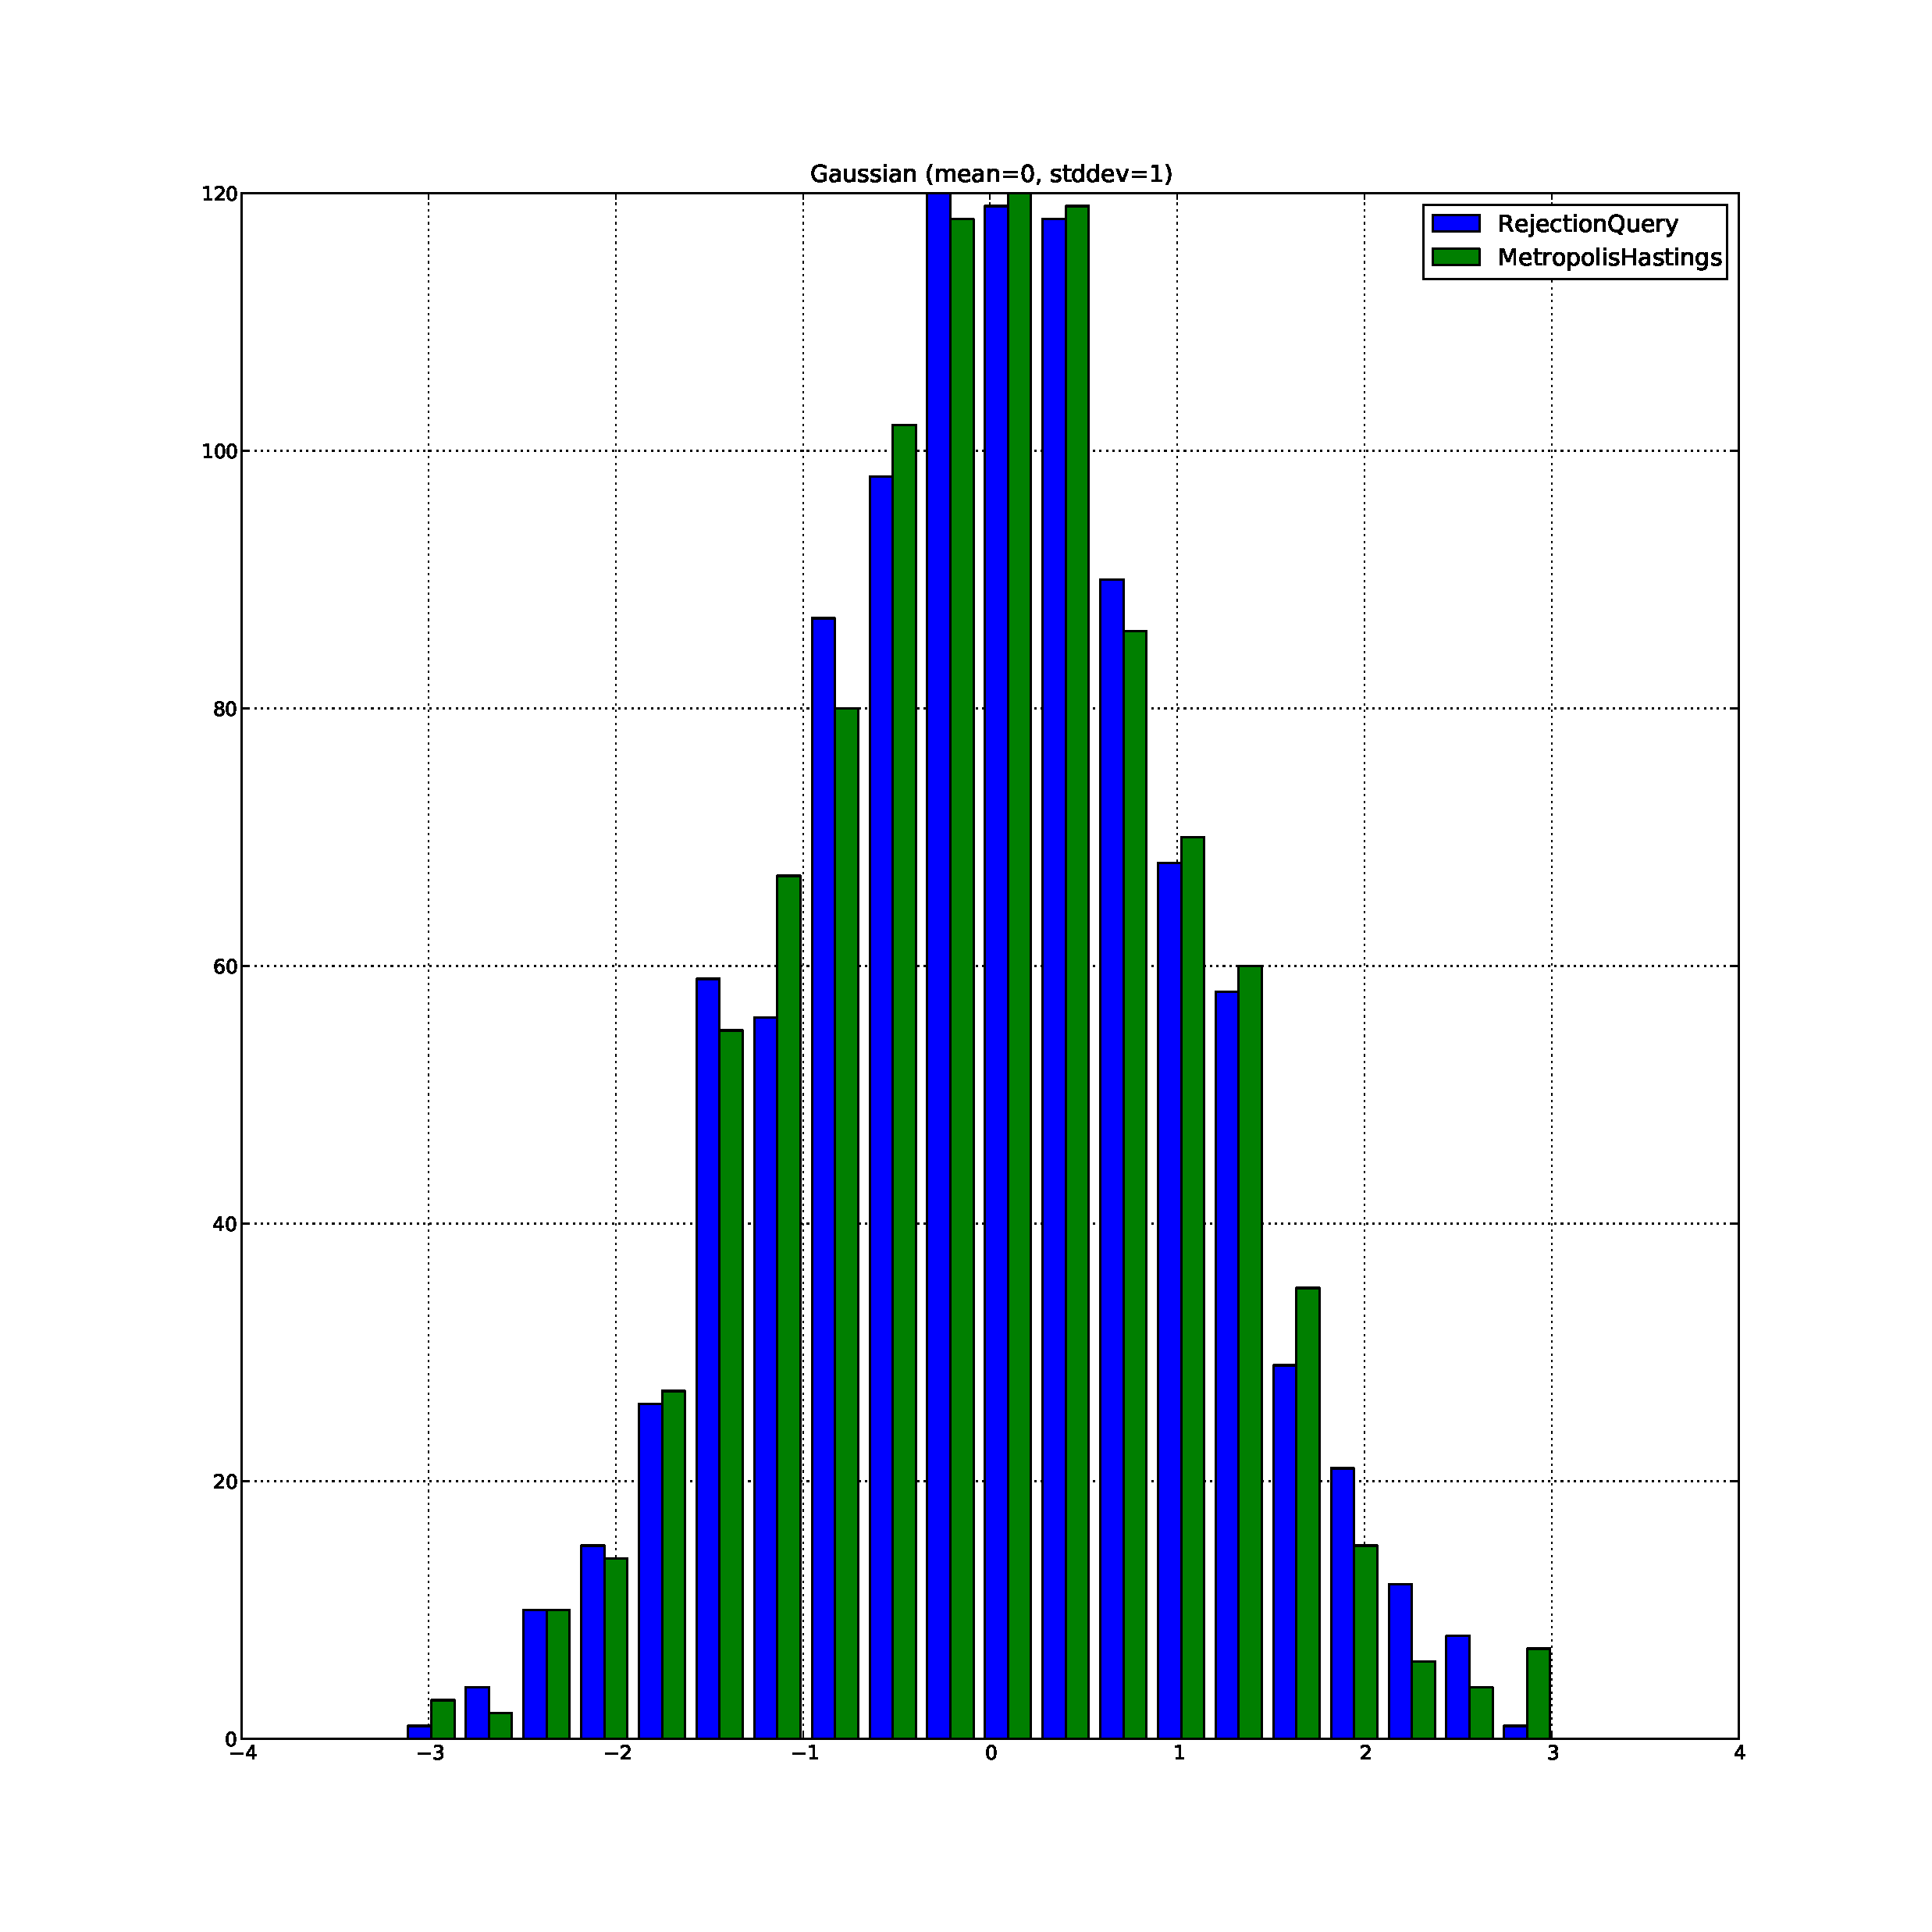
\includegraphics[width=0.33\textwidth]{../graphs/gaussian.pdf}}
\subfloat[Poisson ($\lambda=4$)]{\label{fig:poisson}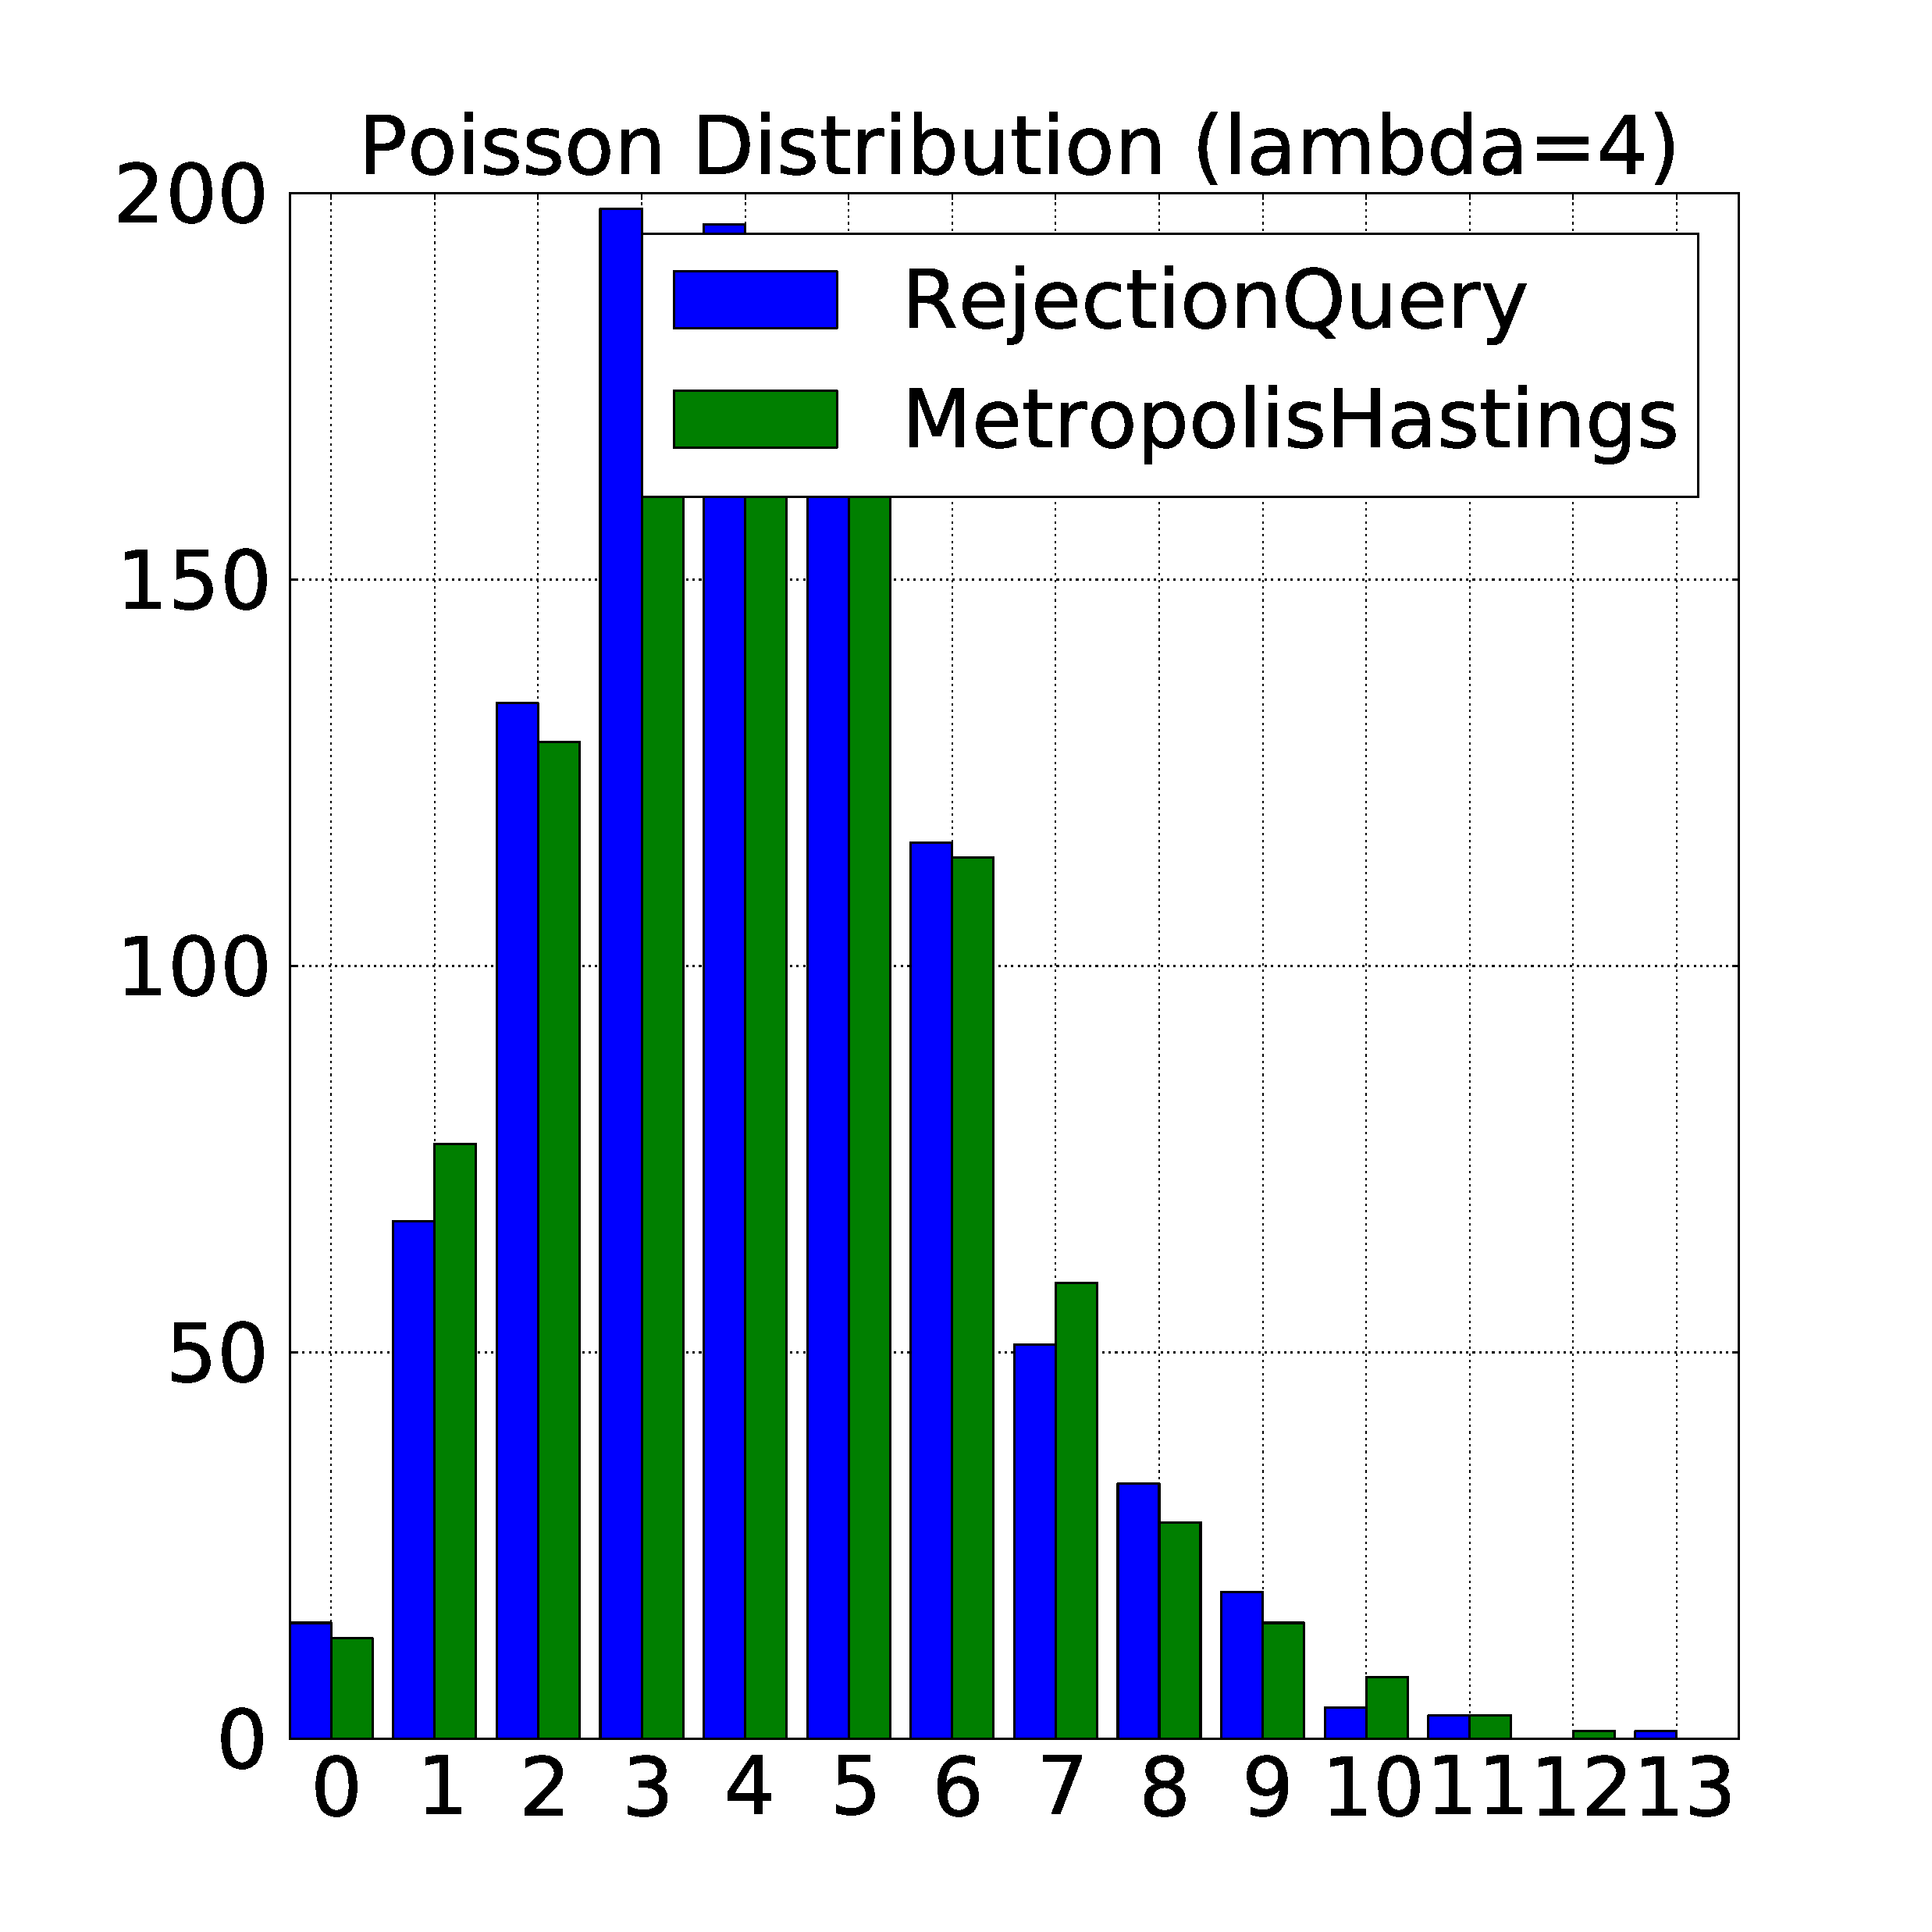
\includegraphics[width=0.33\textwidth]{../graphs/poisson.pdf}}

\subfloat[Sample Integer]{\label{fig:sample_integer}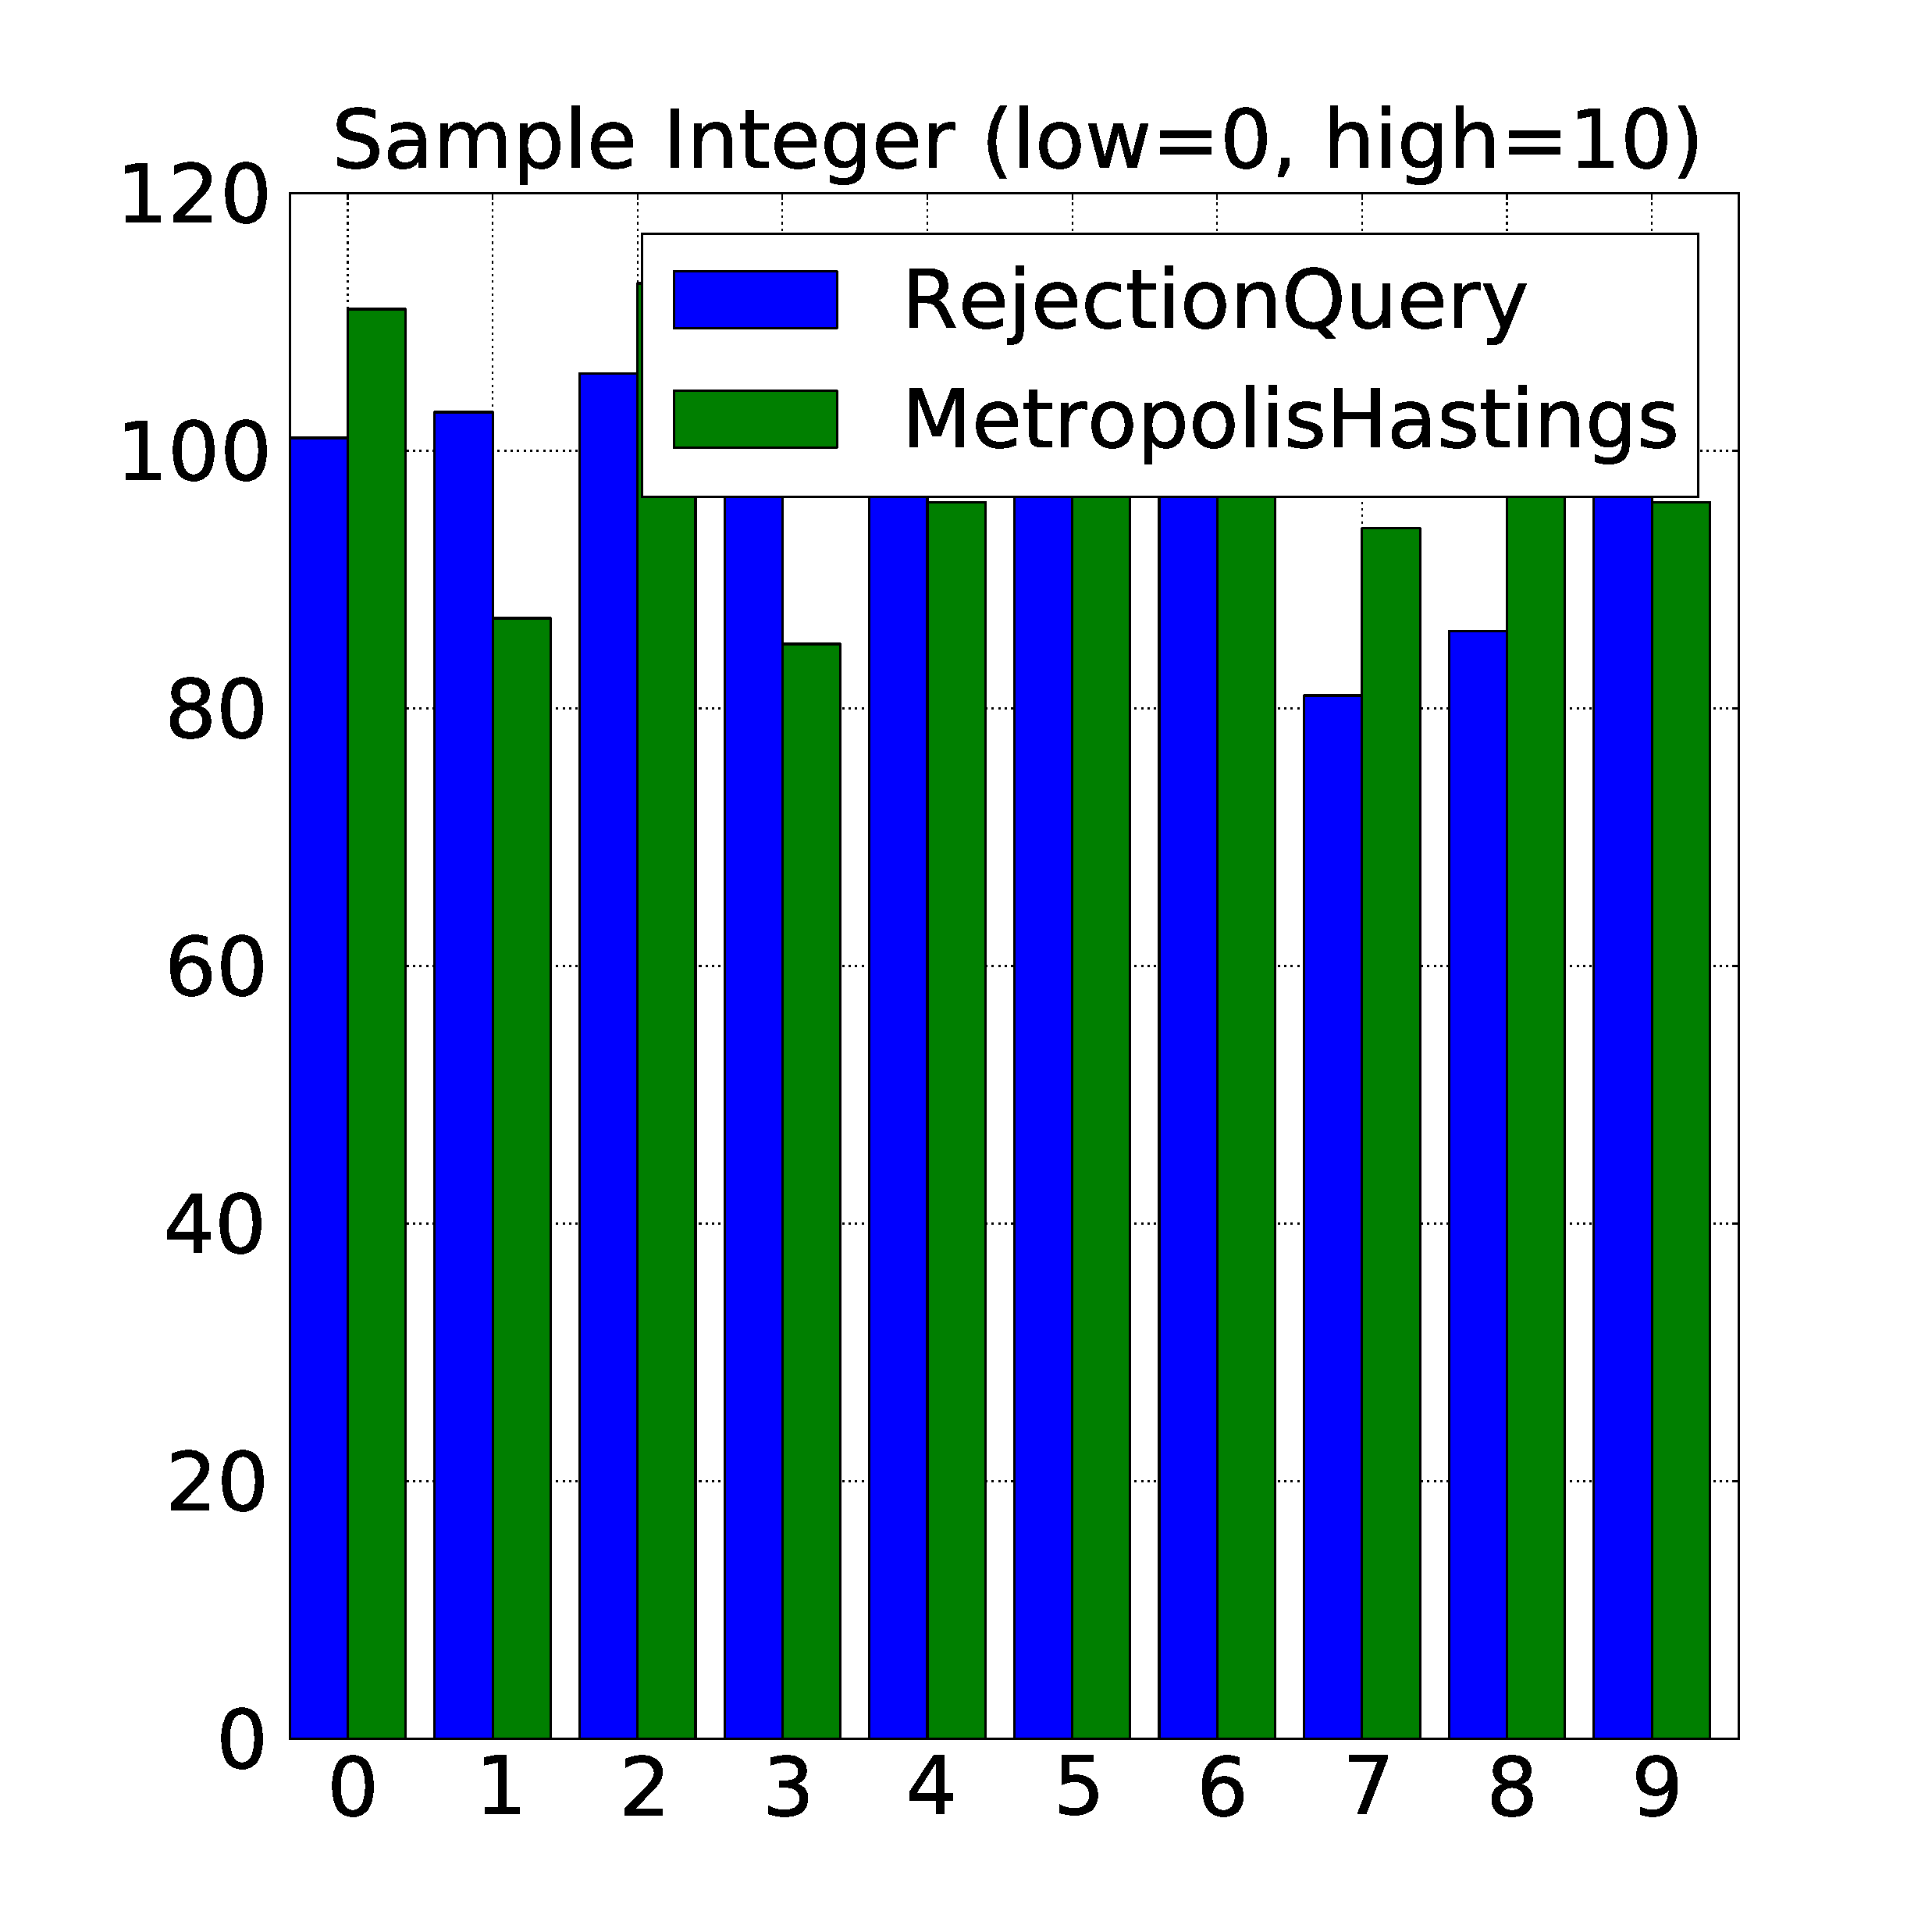
\includegraphics[width=0.33\textwidth]{../graphs/sample_integer.pdf}}
\subfloat[Uniform]{\label{fig:uniform}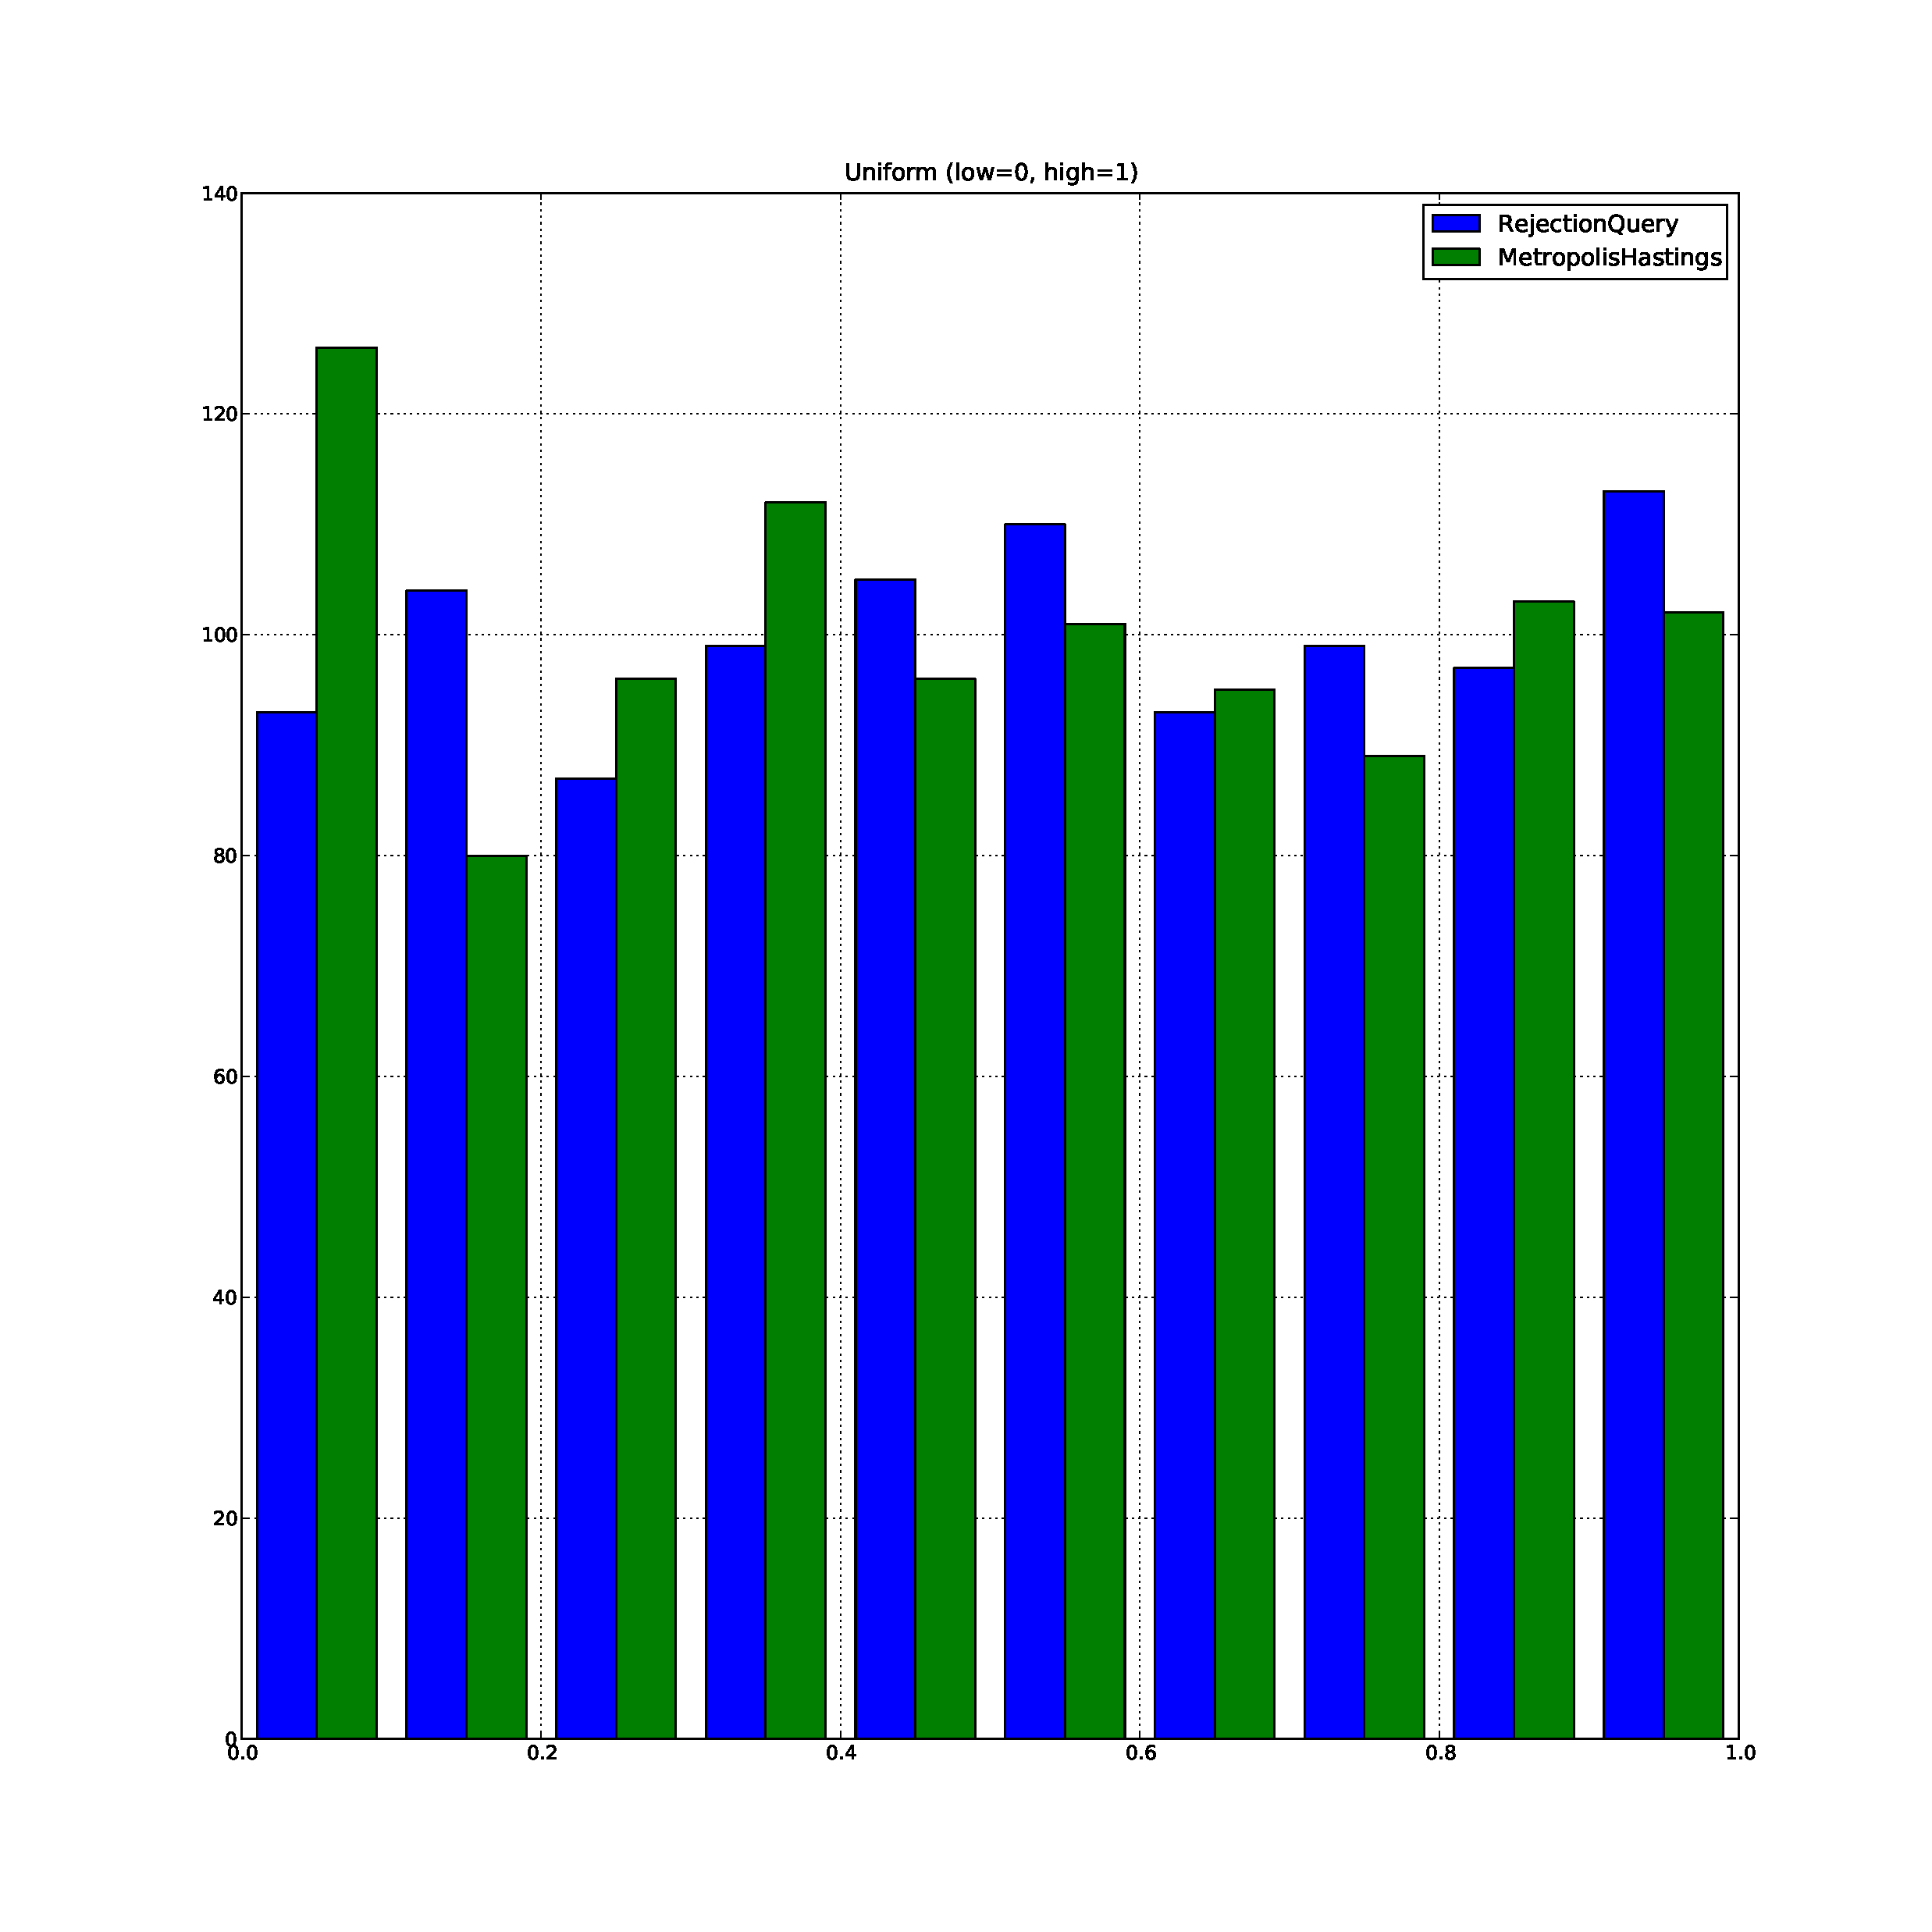
\includegraphics[width=0.33\textwidth]{../graphs/uniform.pdf}}
\caption{\small\textbf{Elementary Random Primitives.}  Both
  \texttt{RejectionQuery} and \texttt{MetropolisHastings} inference
  queries were run to sample the various ERPs.  Both types of queries
  returned distributions are consistent with each other and with the
  original distributions.}
\label{fig:erps}
\end{figure}

The results of these queries are shown in Fig. \ref{fig:models}.  The
first two models were computed withe both \texttt{RejectionQuery} and
\texttt{MetropolisHastings}, while the remaining three were only run
with \texttt{MetropolisHastings}.  All of these results are consistent
with those returned by a Church version of the same model, verifying
that the Metropolis-Hastings algorithm is correctly implemented and
that PyStoch inference works as intended.

\begin{figure}
\centering
\subfloat[\textbf{Basic Conditional Inference.}  The probability that $A=0$ or $A=1$ Given that $D\geq 2$.]{\label{fig:test1results}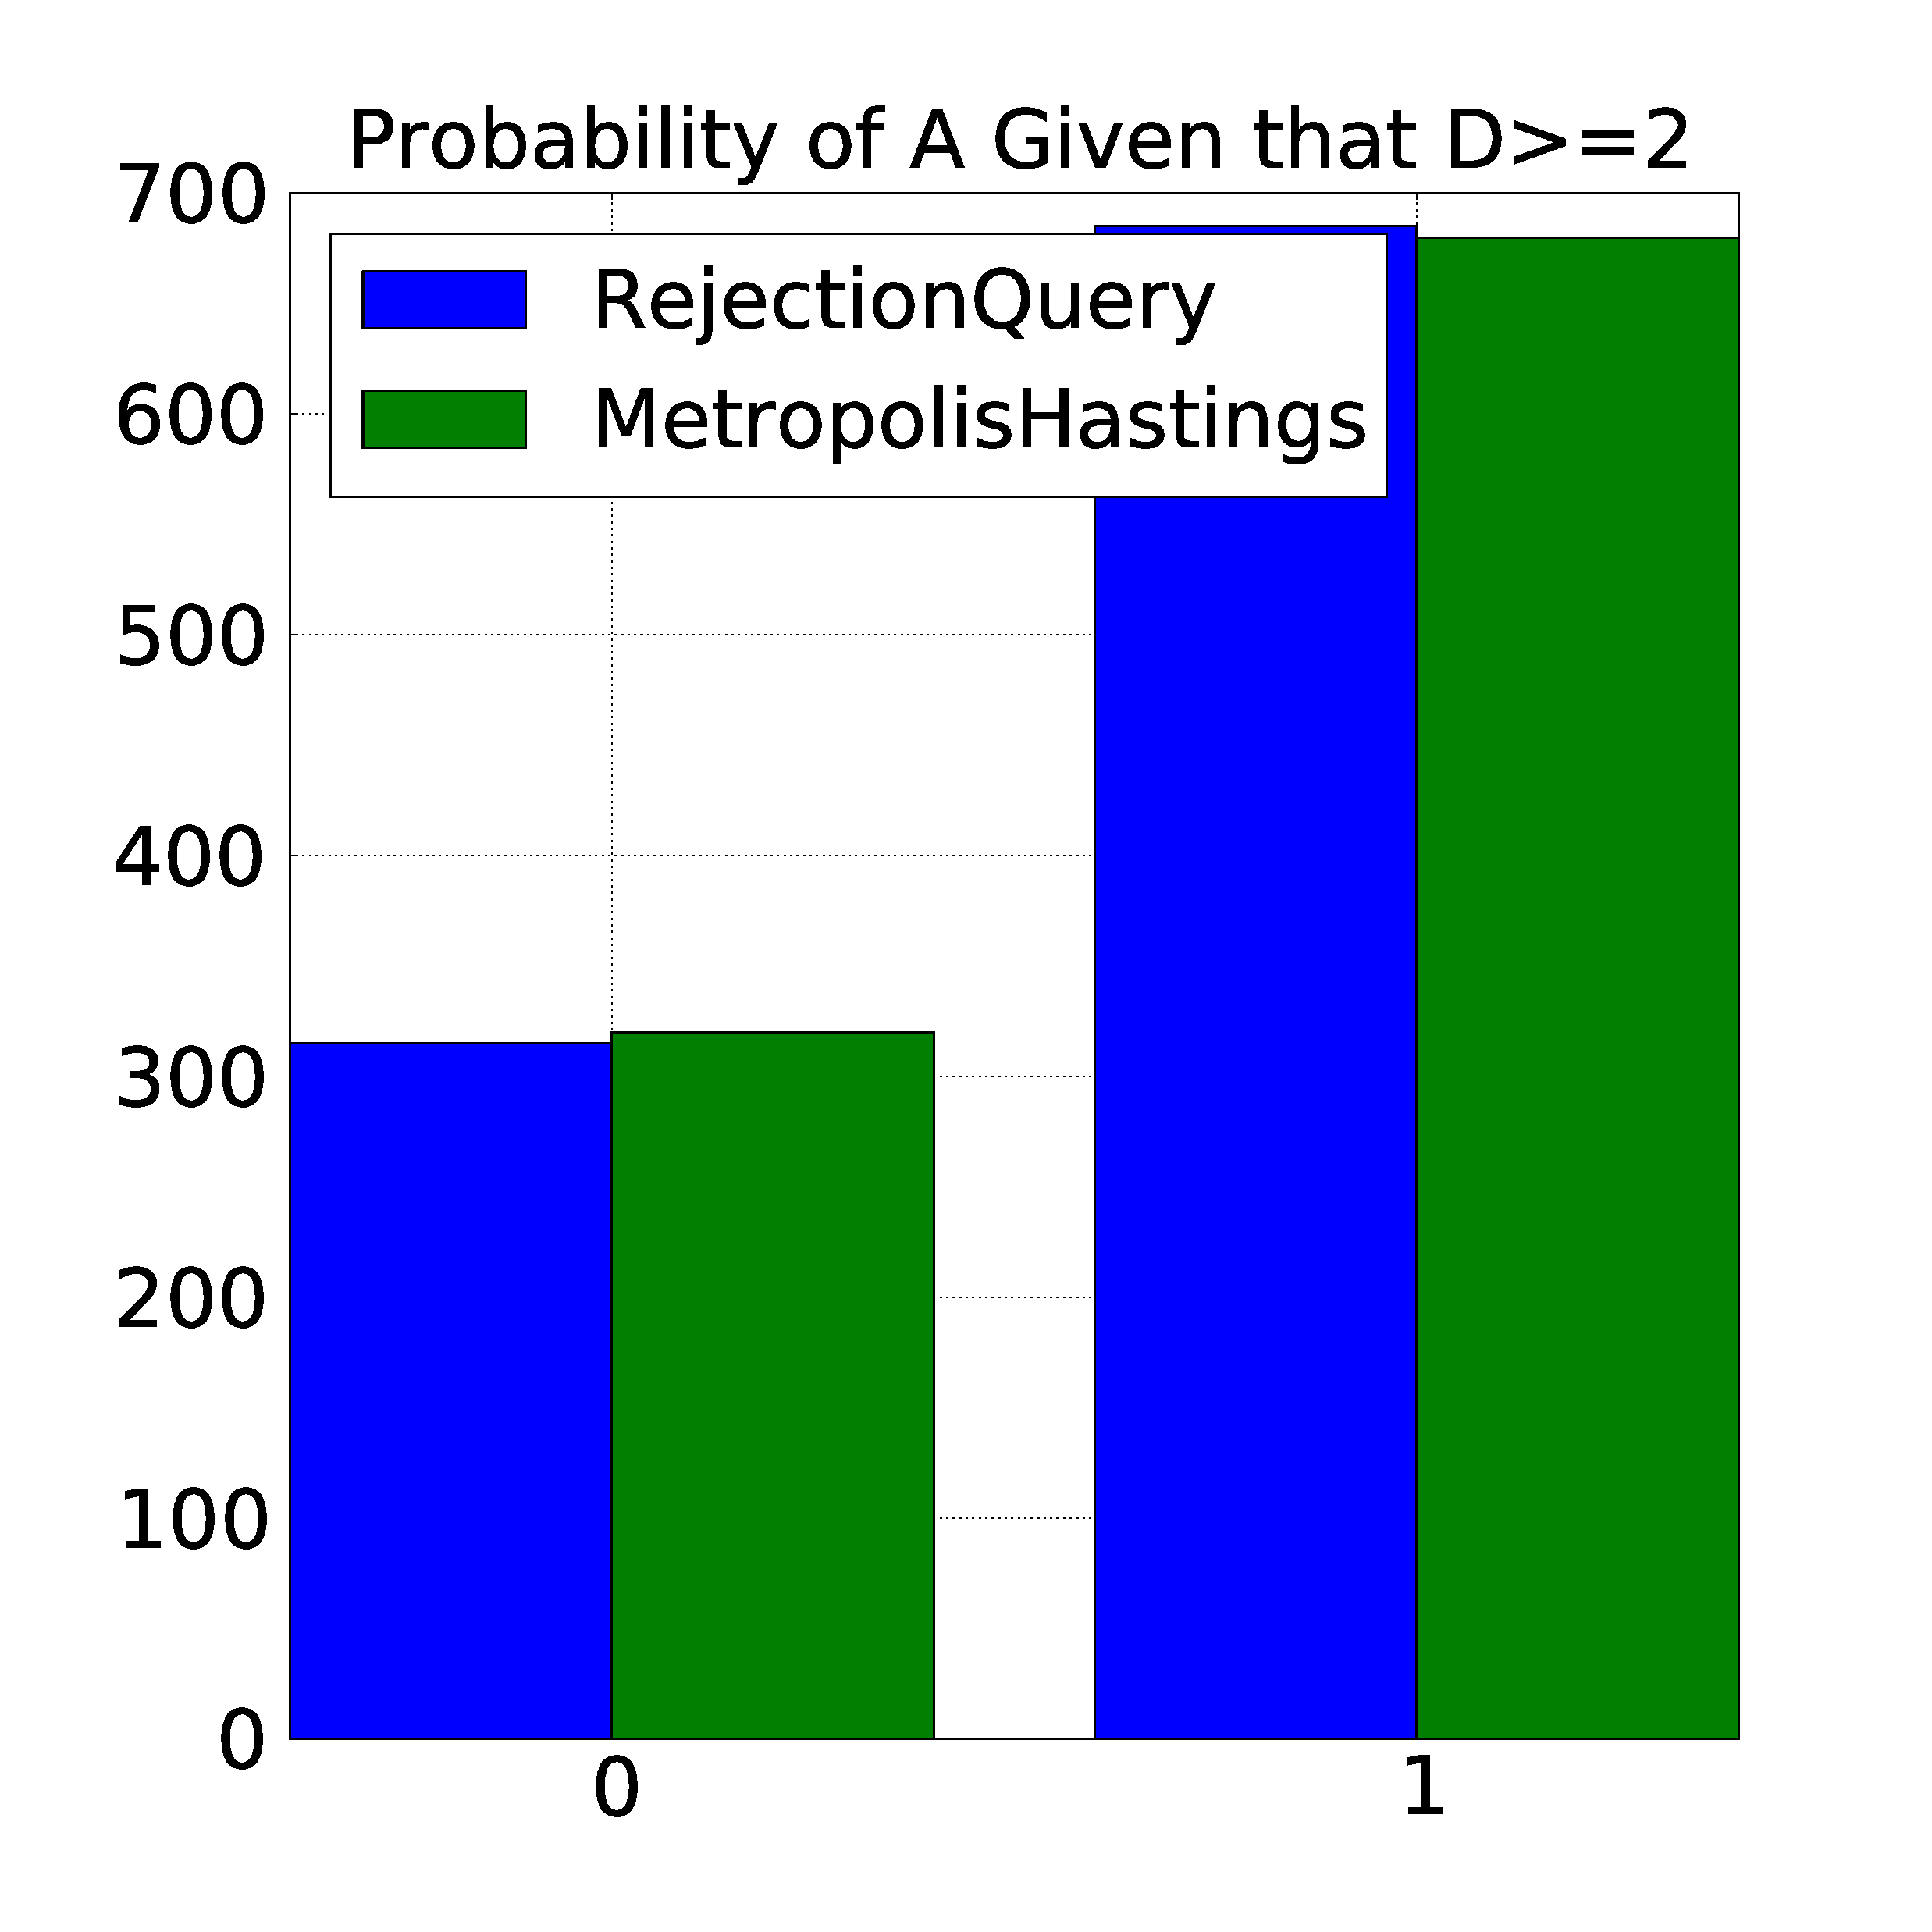
\includegraphics[width=0.33\textwidth]{../graphs/test1.pdf}}
\hspace{40pt}
\subfloat[\textbf{Breast Cancer.}  The probability of having breast cancer given a positive mammogram.]{\label{fig:test2results}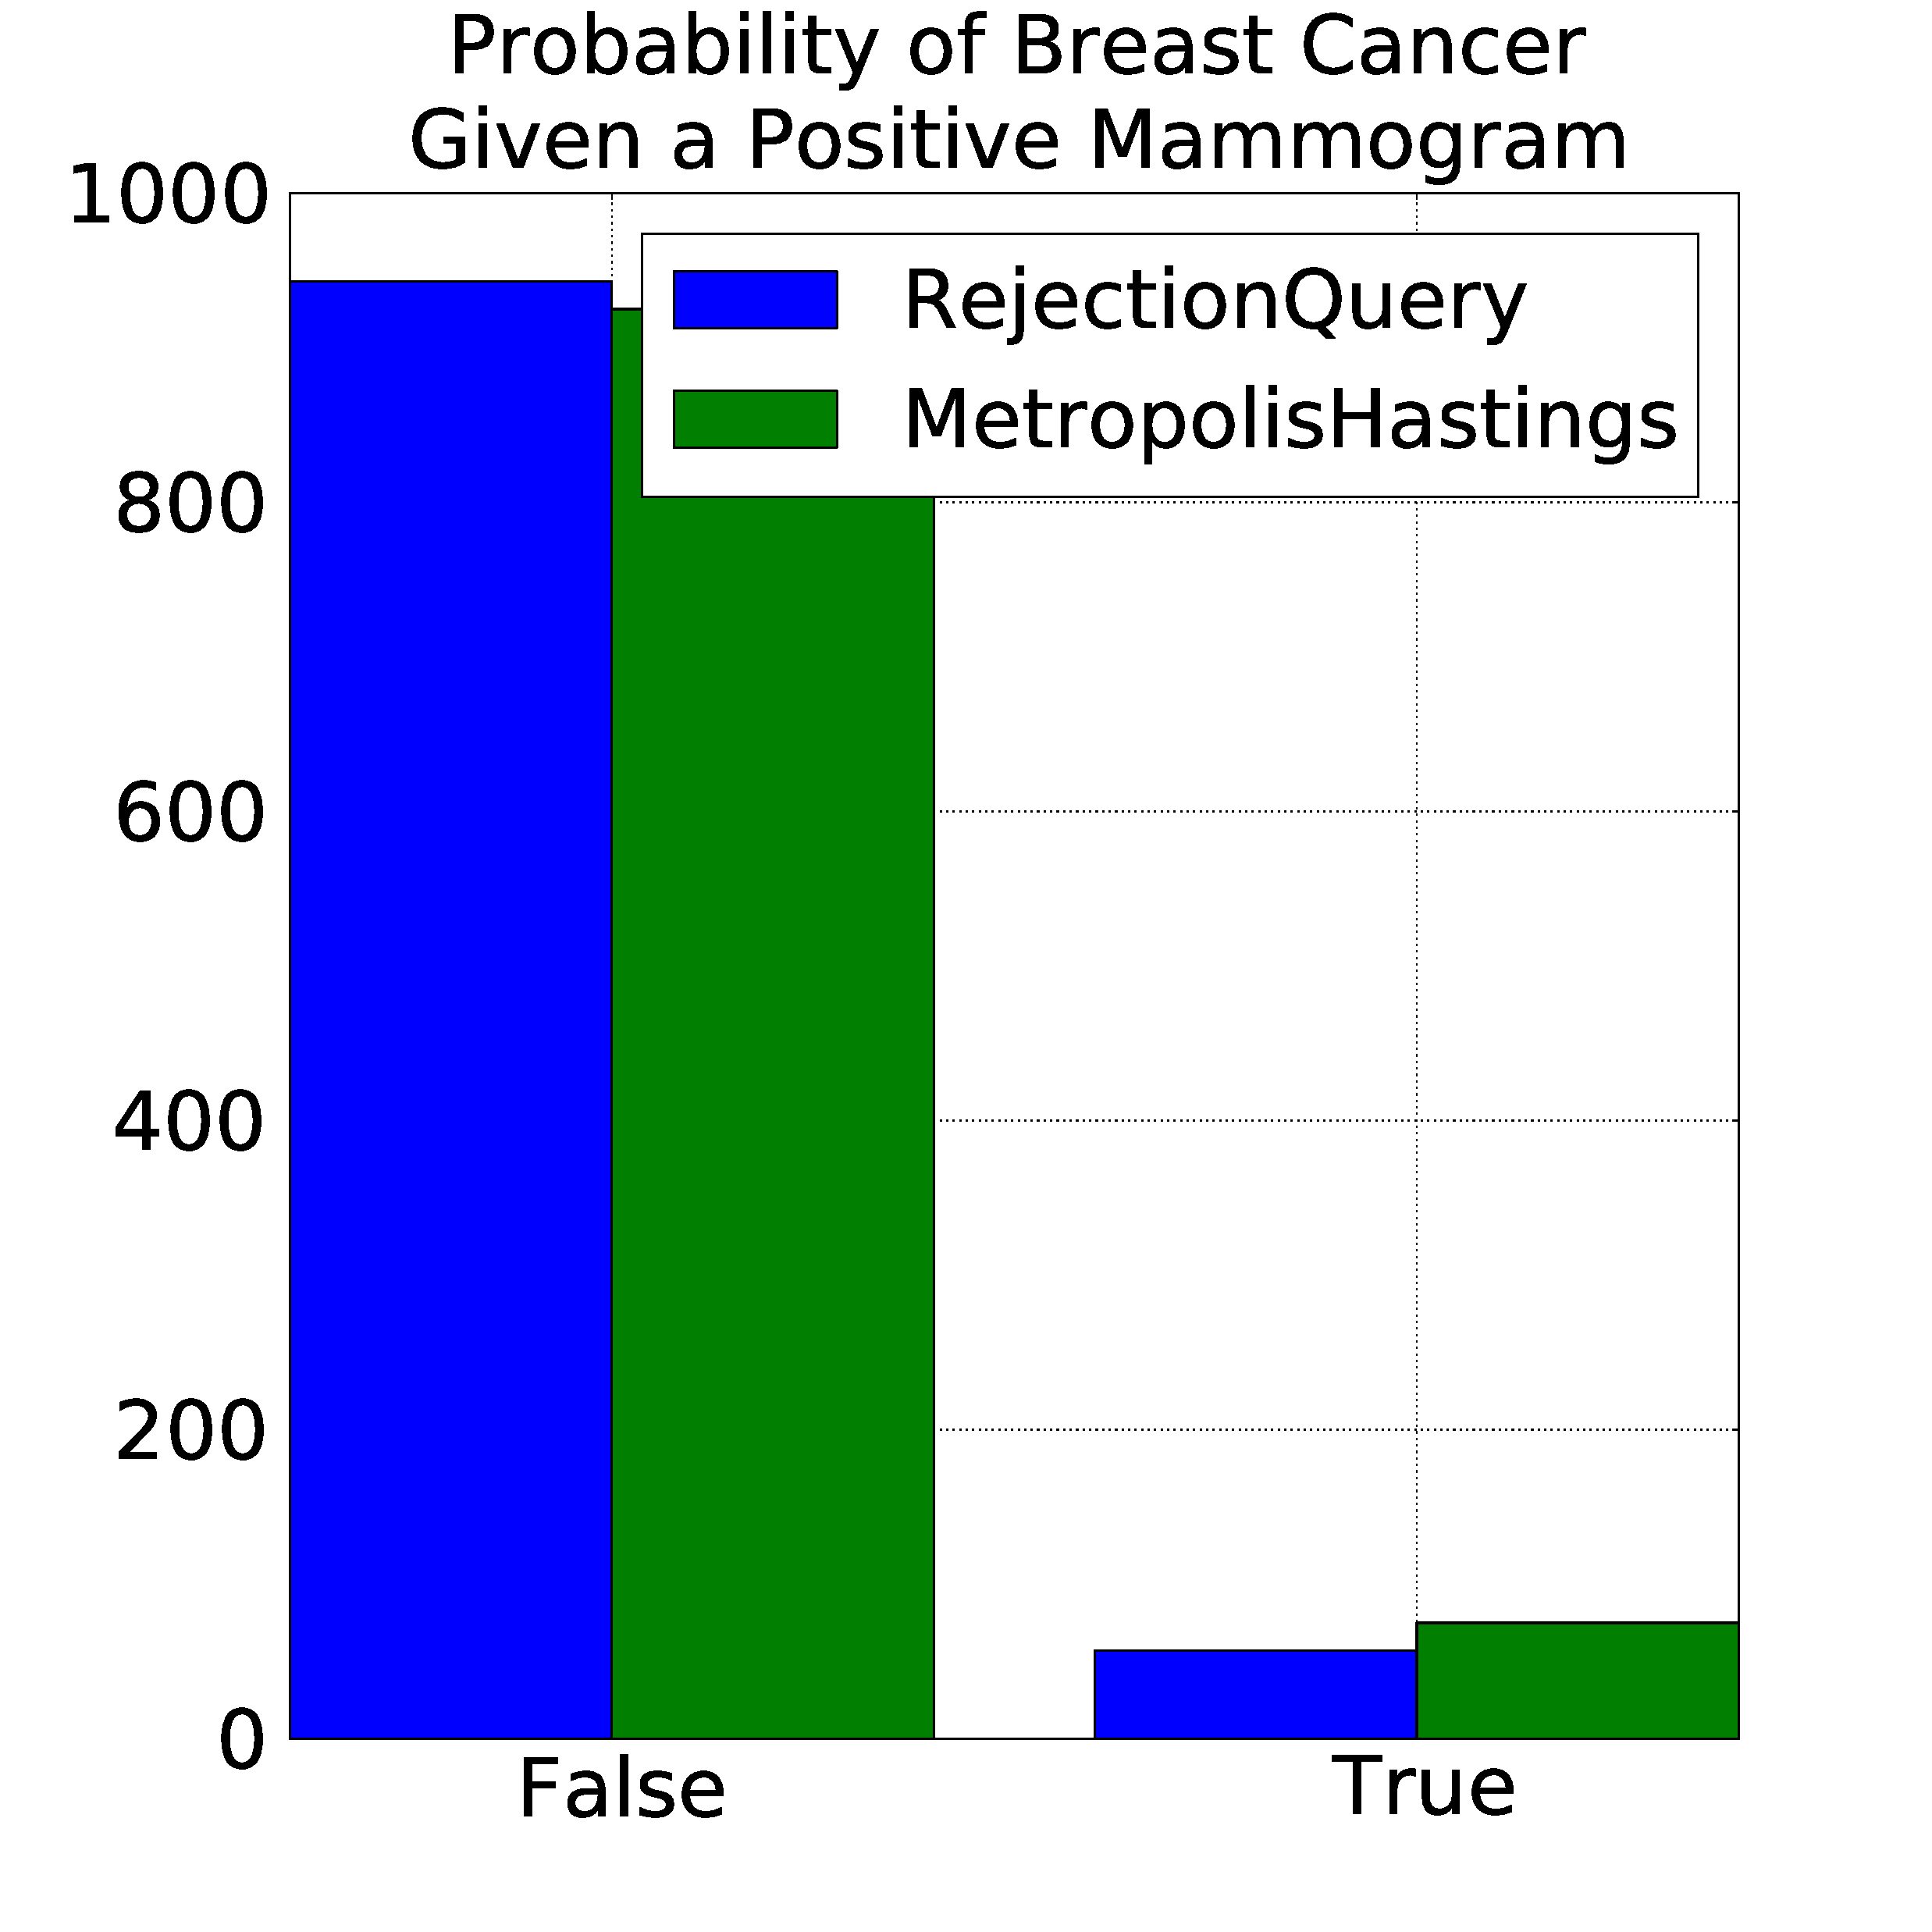
\includegraphics[width=0.33\textwidth]{../graphs/test2.pdf}}

\subfloat[\textbf{Joint Inferences for Lung Cancer and TB.}  The probability of having lung cancer and/or TB given a cough, fever, chest pain, and shortness of breath.]{\label{fig:test3results}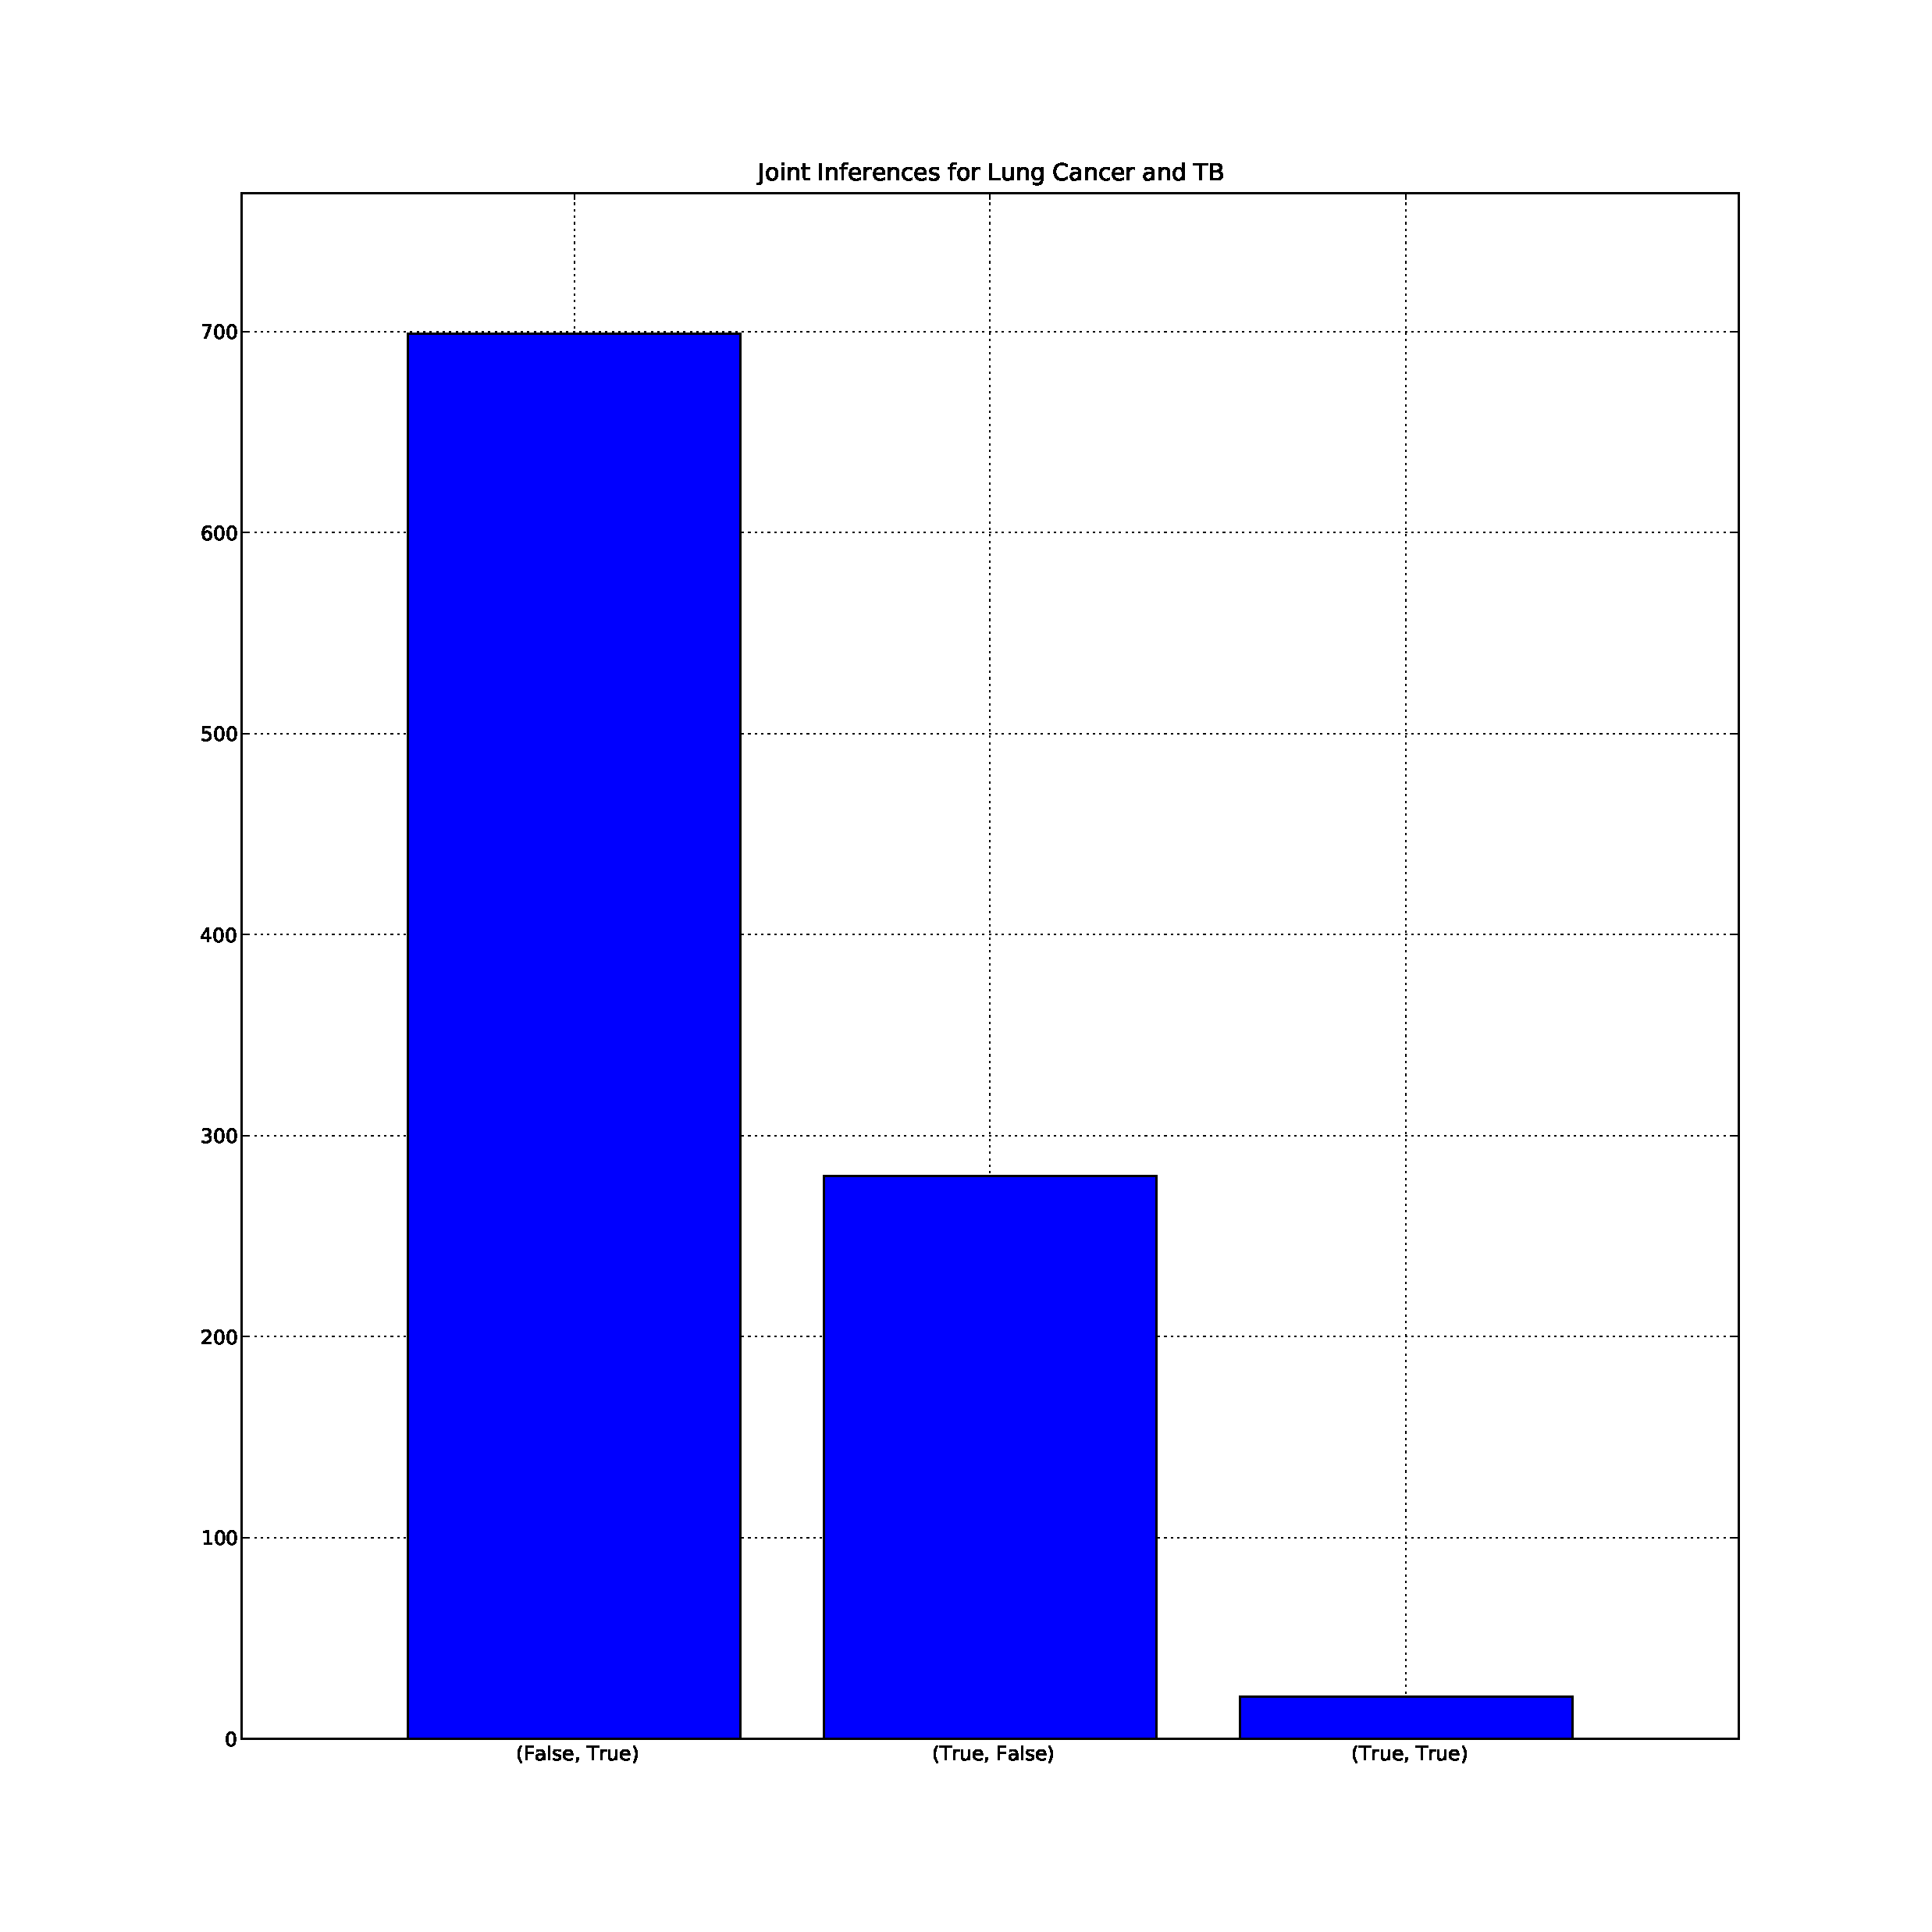
\includegraphics[width=0.33\textwidth]{../graphs/test3.pdf}}
\hspace{40pt}
\subfloat[\textbf{Coin Weight.}  Beliefs about the weight of a coin before and after observing the sequence $\{H,H,H,H,H\}$.]{\label{fig:test4results}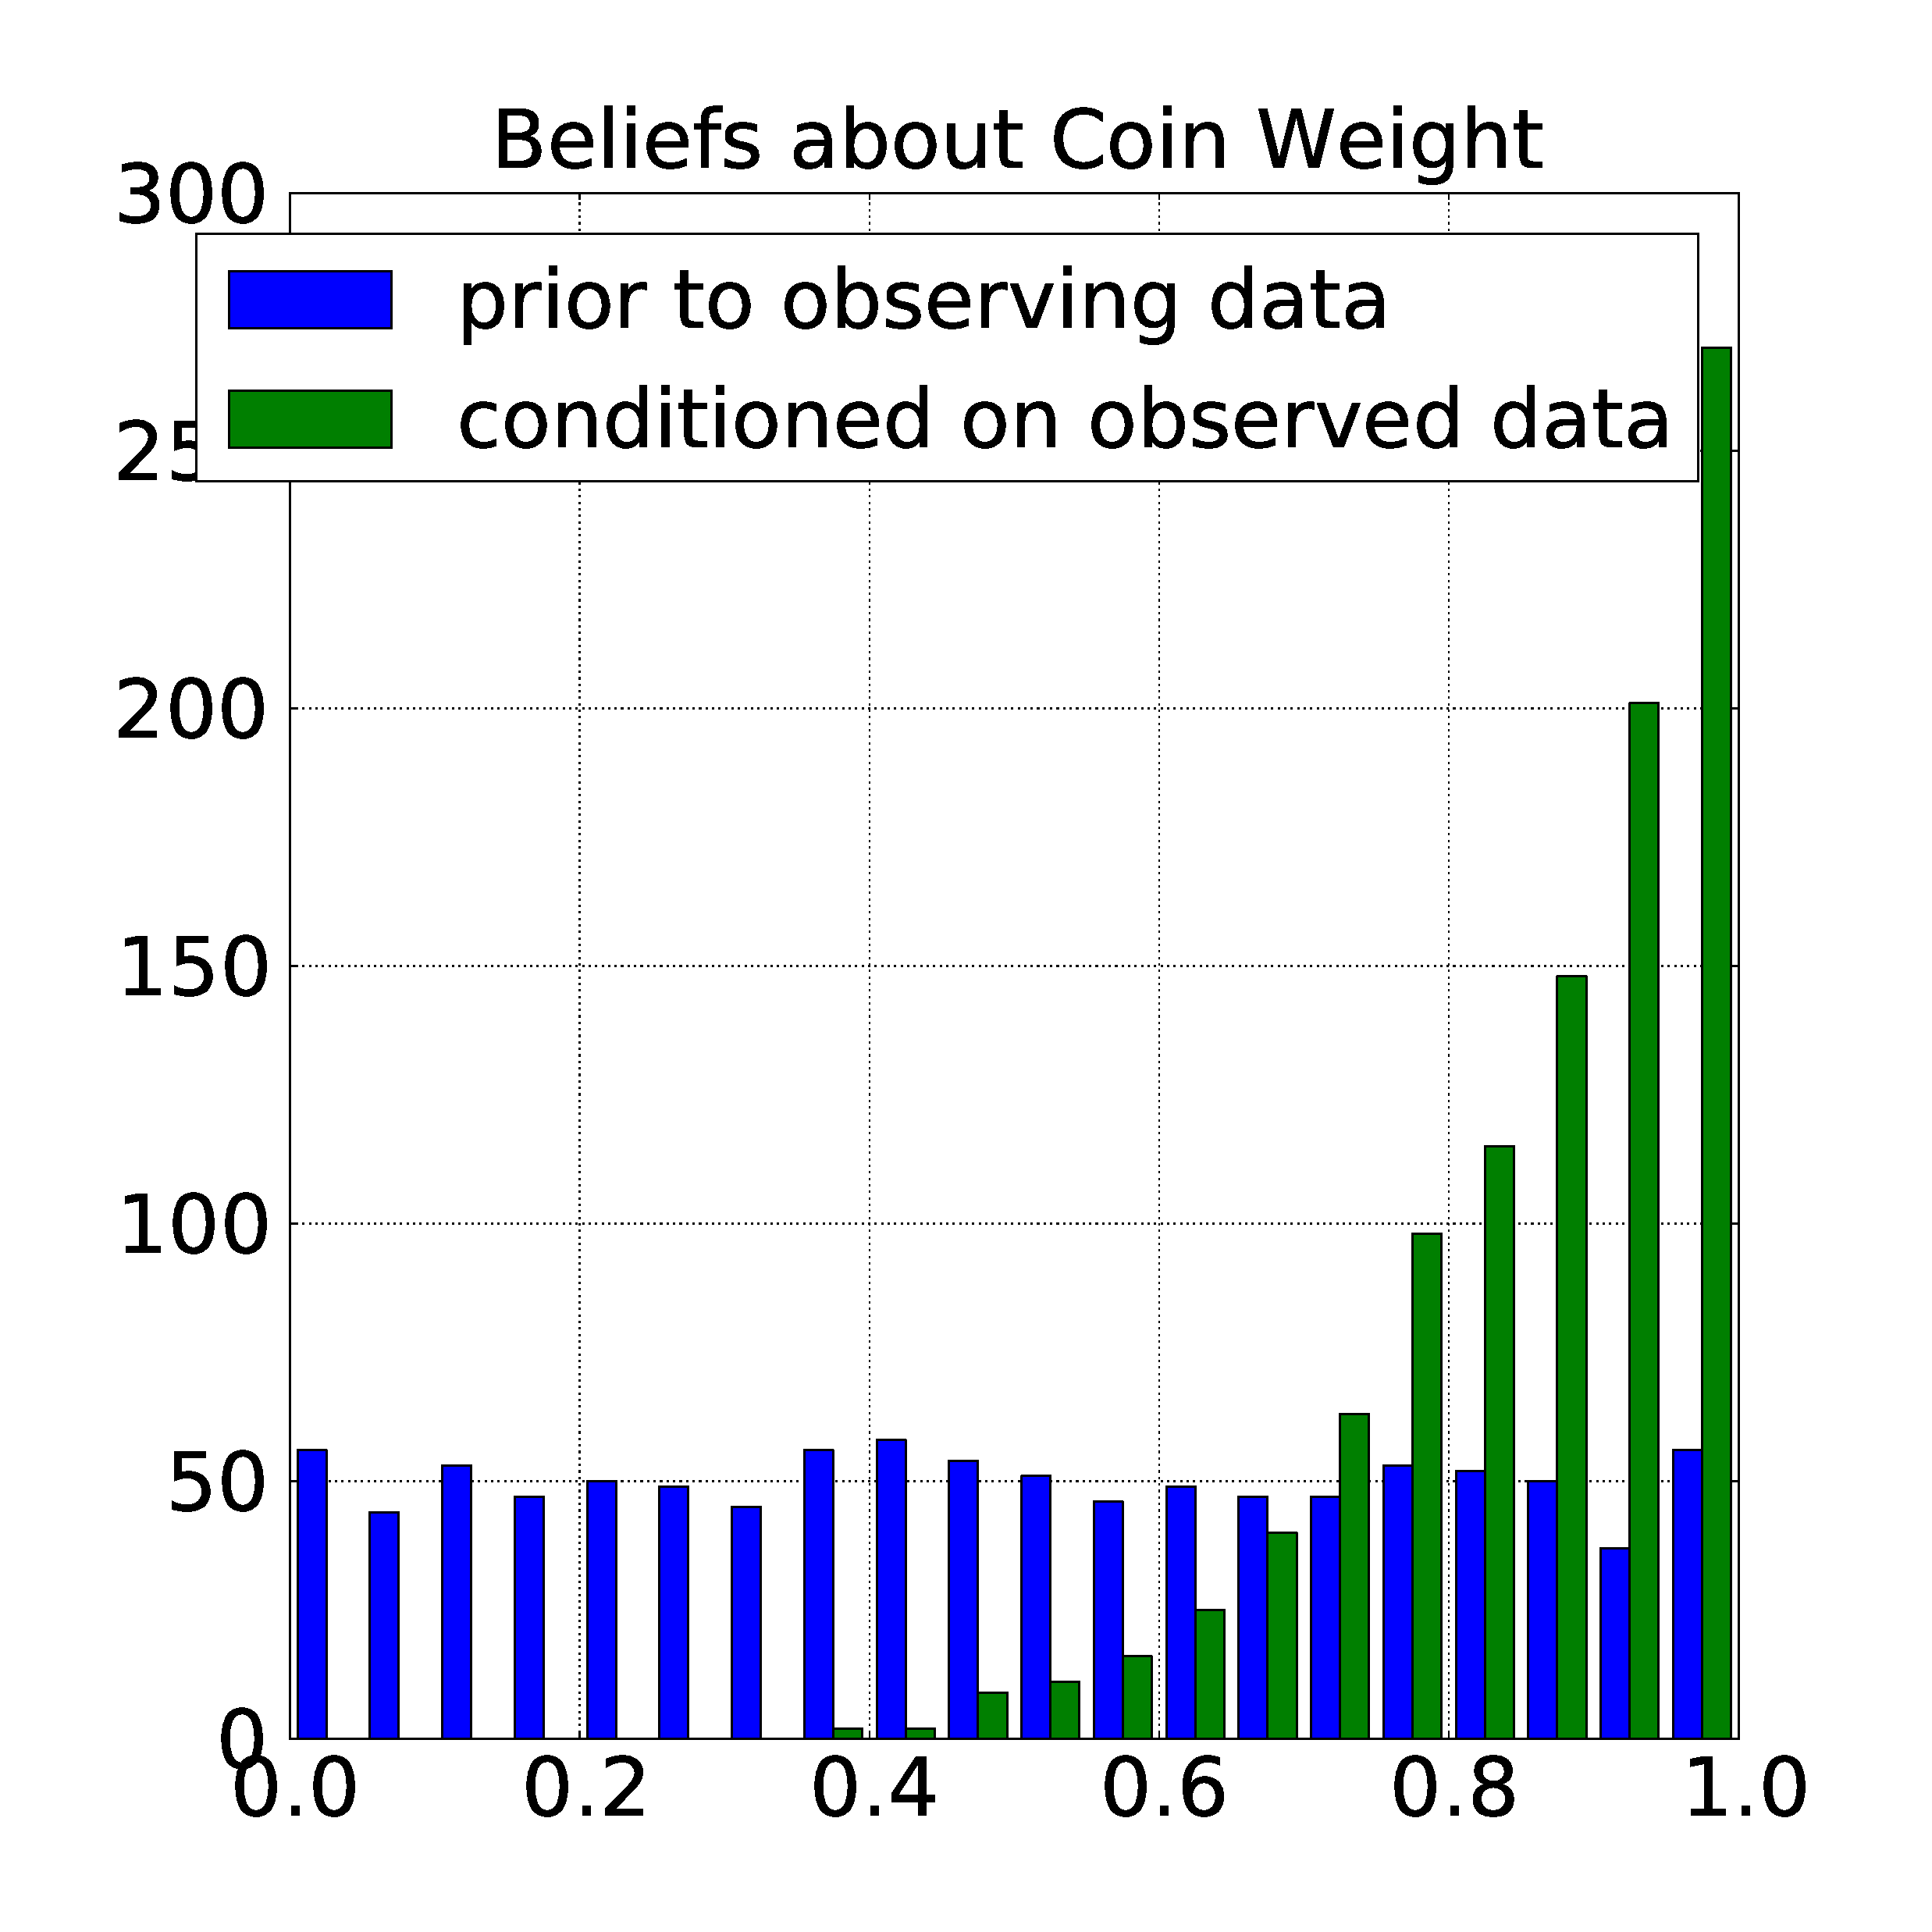
\includegraphics[width=0.33\textwidth]{../graphs/test4.pdf}}

\subfloat[\textbf{Occam's Razor.}  The probability that a set of data was taken from a large vs. small super set.]{\label{fig:test5results}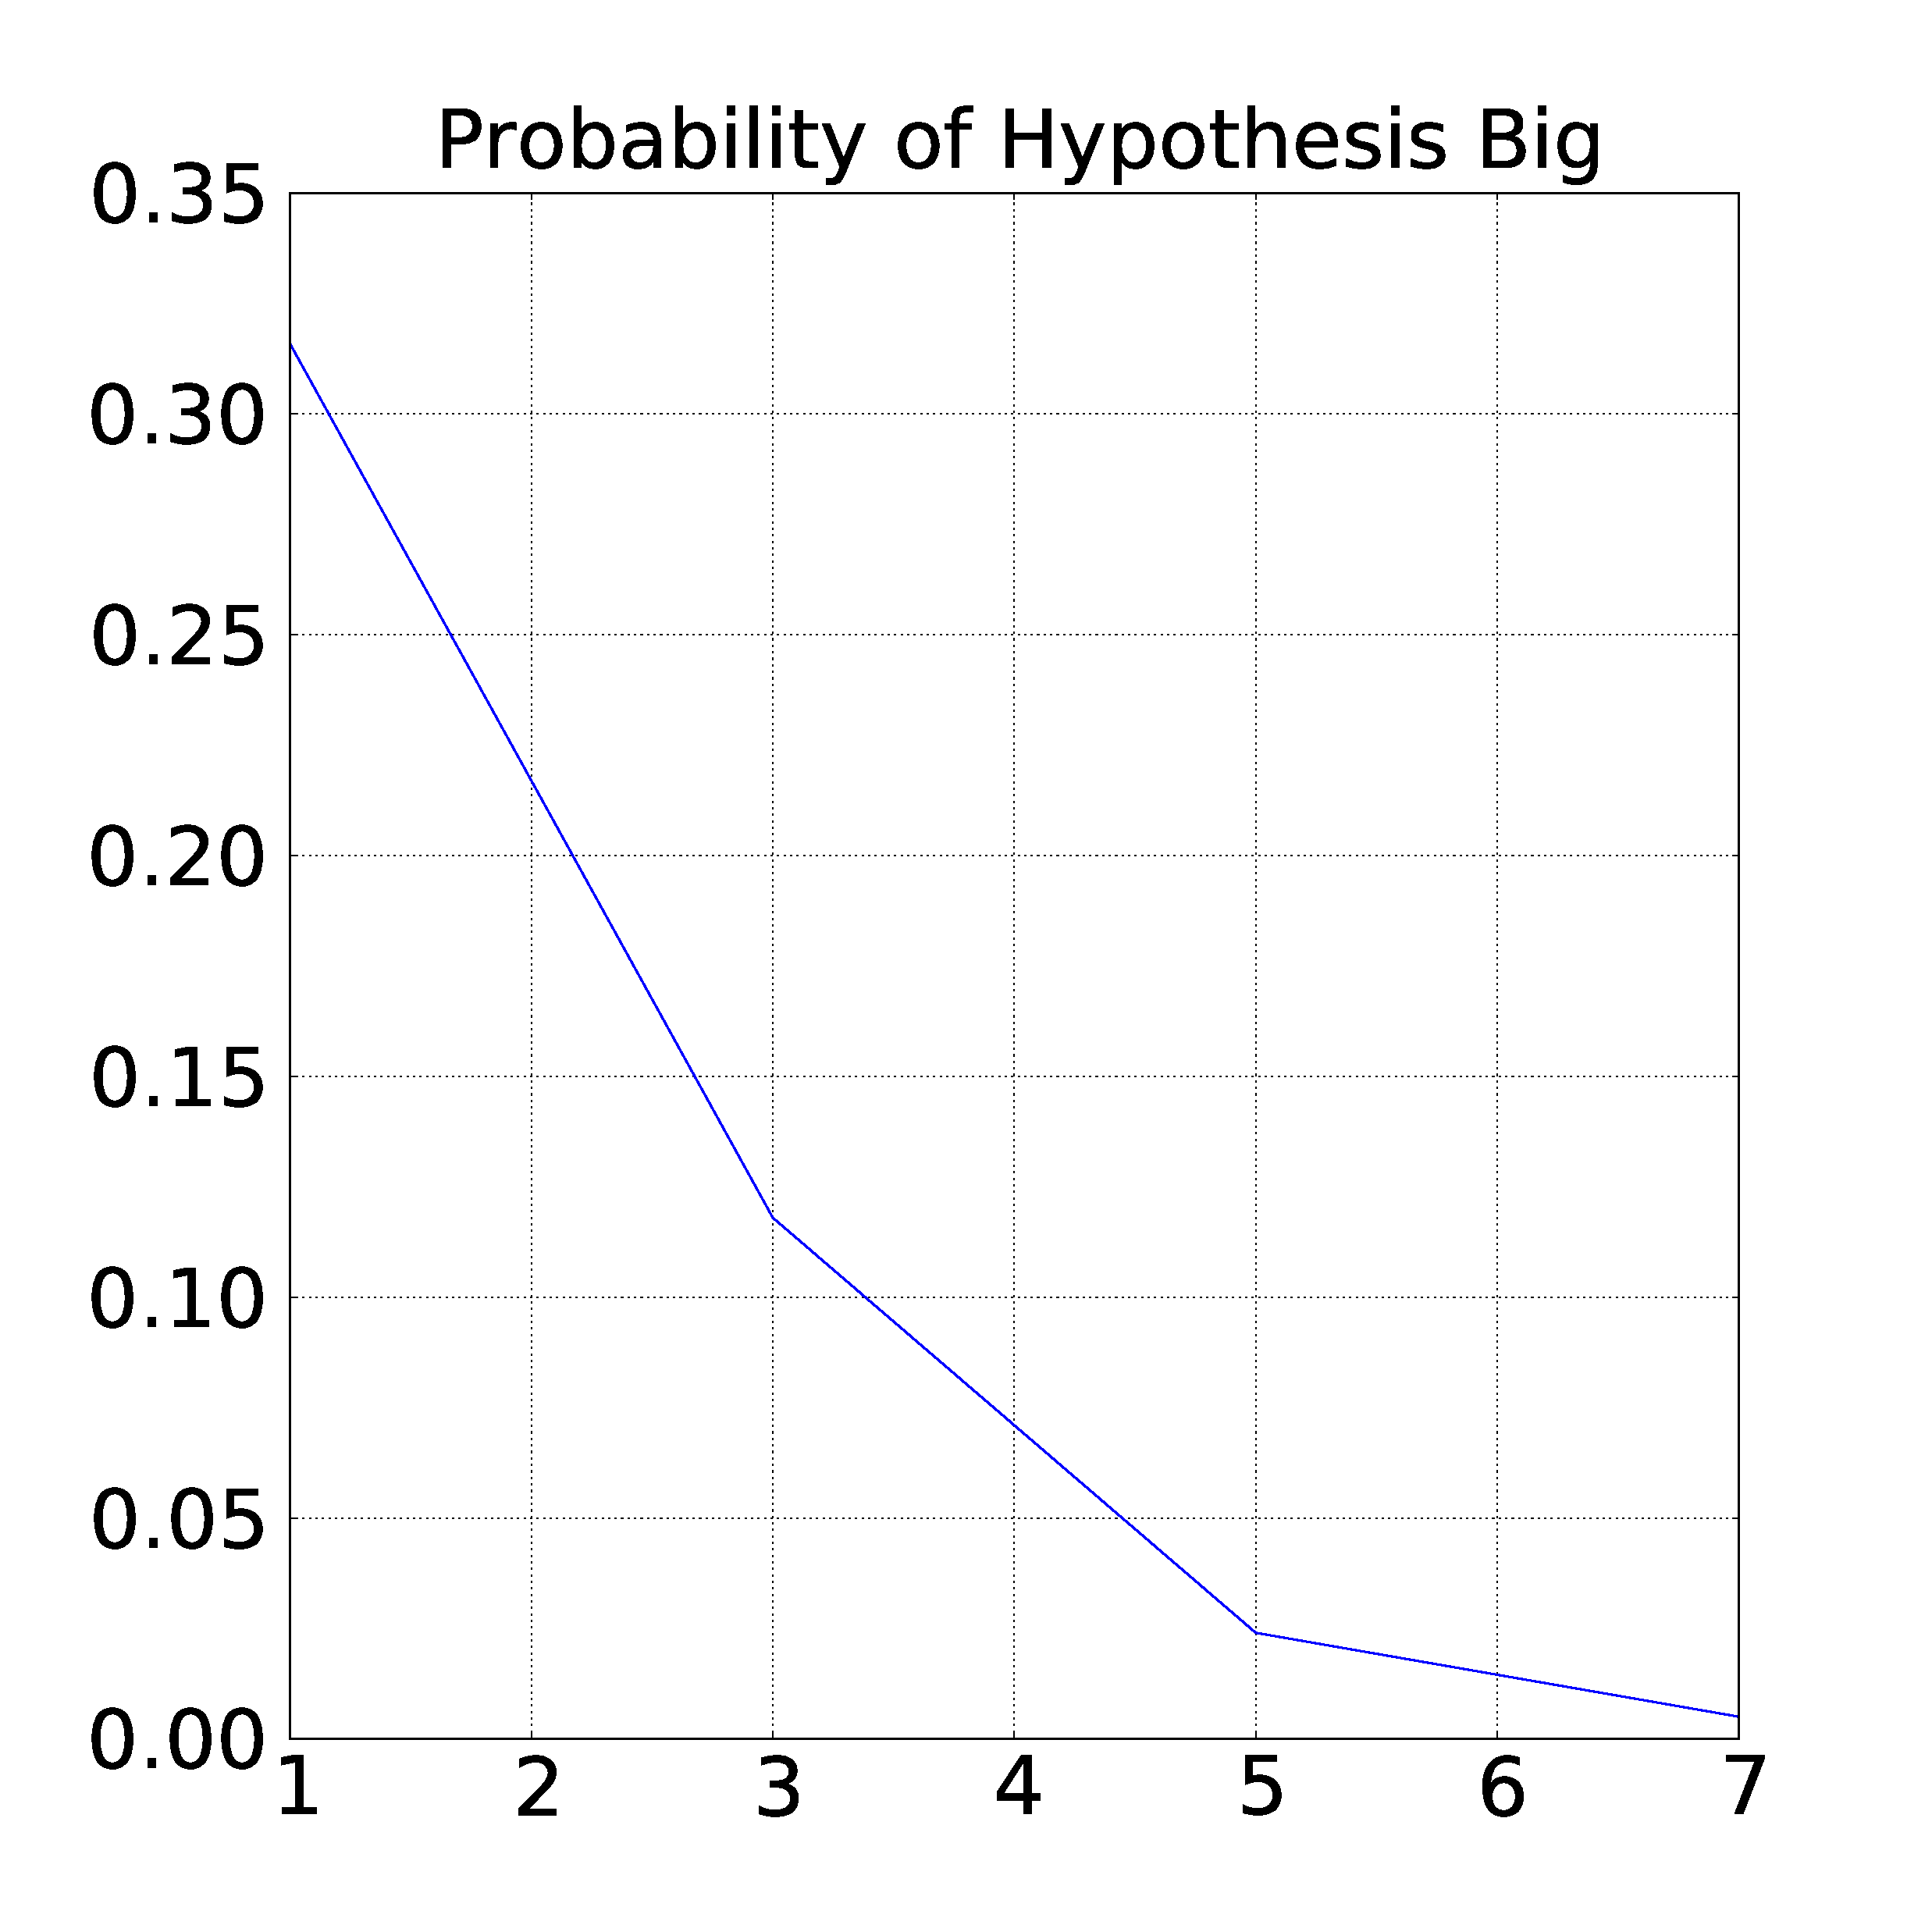
\includegraphics[width=0.33\textwidth]{../graphs/test5.pdf}}
\caption{\small\textbf{Model Results.}}
\label{fig:models}
\end{figure}

\section{Future Improvements}

While PyStoch can currently be used in many situations for many
different types of models, there are several features yet to be
implemented.  The most glaring of these is the lack of memoization.
Church provides the useful feature of being able to memoize (store)
the value of a random variable such that it does not change between
traces of the program.  PyStoch currently has no support for this.

There are also several features of the Python language which are not
supported, most notably \texttt{lambda} functions.  It is not
immediately clear what the best way to rewrite lambdas would be: there
can easily be nested functions within a lambda, but in Python lambdas
may only be on a single line.  The best way of dealing with this issue
is likely to actually create a real function in place of the lambda,
but this approach feels very rough around the edges.  Other Pythonic
features not currently supported are generators, set comprehensions,
dictionary comprehensions, and the \texttt{pass} keyword.
Additionally, Python 2.6 is the only version currently compatible with
PyStoch.  In the future, PyStoch will gain support for Python 2.7 and
Python 3.0; the missing features in the code transformation will
likely be implemented at that time.

One of the biggest complaints of Python in general is its slowness as
a language.  This is due to the fact that it is an interpreted, as
opposed to compiled, language.  The overhead of the extra function
calls needed to support \texttt{MetropolisHastings} certainly does not
help the speed of PyStoch queries.  Future work on PyStoch will
examine the profiles of various models and examine ways of speeding up
the computation, possibly making use of threads and lazy evaluation.

\section{Conclusion}

PyStoch proved to be a fairly straightforward implementation of the
imperative probabilistic programming framework as defined by
\citeA{Wingate2011}.  Its true power lies not in the
Metropolis-Hastings inference alone, but in the combination of such
queries with the countless number of external libraries available to
Python coders.  For example, the \texttt{numpy}, \texttt{scipy}, and
\texttt{matplotlib} libraries provide powerful tools for manipulating
arrays of data, performing data analysis, and graphing results.
Scheme, unfortunately, does not have such easy access to similar
interfaces, making it difficult to actually use the data generated
from Church models.  Matlab has similar capabilities to the libraries
mentioned above, but falls short in other areas, such as graphics.

PyStoch is a work in progress, but even this initial implementation
may prove to be a useful tool to Python programmers wishing to perform
inference.  Through future addition of features and research in
general surrounding probabilistic programming, PyStoch will become an
even more powerful resource for researchers who need both a flexible
coding environment and robust inference engine.

\bibliographystyle{apacite}

\setlength{\bibleftmargin}{.125in}
\setlength{\bibindent}{-\bibleftmargin}

\bibliography{pystoch}

\newpage
\section{Appendix}

\begin{figure}[h!]
\begin{verbatim}
class Query():

    def __init__(self):
        self.baserate = 0.1

    def query_model(self):
        self.A = int(flip(self.baserate))
        self.B = int(flip(self.baserate))
        self.C = int(flip(self.baserate))
        self.D = self.A + self.B + self.C

    def sample(self):
        return self.A

    def condition(self):
        return self.D >= 2
\end{verbatim}
\caption{\small\textbf{Basic Conditional Inference Model.}}
\label{fig:test1model}
\end{figure}

\begin{figure}[h!]
\begin{verbatim}
class Query():

    def __init__(self):
        return

    def query_model(self):
        self.breast_cancer = flip(0.01)

        if self.breast_cancer:
            self.positive_mammogram = flip(0.8)
        else:
            self.positive_mammogram = flip(0.096)

    def sample(self):
        return self.breast_cancer

    def condition(self):
        return self.positive_mammogram
\end{verbatim}
\caption{\small\textbf{Breast Cancer Inference Model.}}
\label{fig:test2model}
\end{figure}

\begin{figure}[h!]
\begin{verbatim}
class Query():

    def __init__(self):
        return

    def query_model(self):
        self.lung_cancer = flip(0.01)
        self.TB = flip(0.005)
        self.cold = flip(0.2)
        self.stomach_flu = flip(0.1)
        self.other = flip(0.1)

        self.cough = (self.cold and flip(0.5)) or \
                     (self.lung_cancer and flip(0.3)) or \
                     (self.TB and flip(0.7)) or \
                     (self.other and flip(0.01))
        
        self.fever = (self.cold and flip(0.3)) or \
                     (self.stomach_flu and flip(0.5)) or \
                     (self.TB and flip(0.2)) or \
                     (self.other and flip(0.01))

        self.chest_pain = (self.lung_cancer and flip(0.4)) or \
                          (self.TB and flip(0.5)) or \
                          (self.other and flip(0.01))

        self.shortness_of_breath = (self.lung_cancer and flip(0.4)) or \
                                   (self.TB and flip(0.5)) or \
                                   (self.other and flip(0.01))

    def sample(self):
        return self.lung_cancer, self.TB

    def condition(self):
        return self.cough and self.fever and \
               self.chest_pain and self.shortness_of_breath
\end{verbatim}
\caption{\small\textbf{Joint Inferences for Lung Cancer and TB.}}
\label{fig:test3model}
\end{figure}

\begin{figure}[h!]
\begin{verbatim}
class Query():

    def __init__(self):
        self.observed_data = ['H', 'H', 'H', 'H', 'H']
        self.num_flips = len(self.observed_data)

    def coin(self, weight):
        if flip(weight):
            return 'H'
        return 'T'

    def query_model(self):
        self.coin_weight = uniform(0, 1)
        self.sampled_data = [self.coin(self.coin_weight) \
                             for i in xrange(self.num_flips)]

    def sample(self):
        return self.coin_weight

    def condition(self):
        return self.observed_data == self.sampled_data
\end{verbatim}
\caption{\small\textbf{Beliefs about Coin Weight.}}
\label{fig:test4model}
\end{figure}

\begin{figure}[h!]
\begin{verbatim}
BIG = 1.0
SMALL = 0.0

class Query():

    global BIG, SMALL

    def __init__(self, data):
        self.data = data[:]
        self.data.sort()

    def hypothesis_set(self, hyp):
        if hyp == BIG:
            return ["a", "b", "c", "d", "e", "f"]
        return ["a", "b", "c"]

    def query_model(self):
        if flip():
            self.hypothesis = BIG
        else:
            self.hypothesis = SMALL

        self.observations = [uniform_draw(self.hypothesis_set(self.hypothesis)) \
                             for i in xrange(len(self.data))]
        self.observations.sort()

    def sample(self):
        return self.hypothesis

    def condition(self):
        return self.observations == self.data
\end{verbatim}
\caption{\small\textbf{Occam's Razor.}}
\label{fig:test5model}
\end{figure}

\end{document}